% 独自のコマンド

% ■ アブストラクト
%  \begin{jabstract} 〜 \end{jabstract}  :日本語のアブストラクト
%  \begin{eabstract} 〜 \end{eabstract}  :英語のアブストラクト

% ■ 謝辞
%  \begin{acknowledgment} 〜 \end{acknowledgment}

% ■ 文献リスト
%  \begin{bib}[100] 〜 \end{bib}


\newif\ifjapanese

\japanesetrue  % 論文全体を日本語で書く(英語で書くならコメントアウト)

\ifjapanese
  \documentclass[a4j,twoside,openright,11pt]{jreport} % 両面印刷の場合。余白を綴じ側に作って右起こし。
  %\documentclass[a4j,11pt]{jreport}                  % 片面印刷の場合。
  \renewcommand{\bibname}{参考文献}
  \newcommand{\acknowledgmentname}{謝辞}
\else
  \documentclass[a4paper,11pt]{report}
  \newcommand{\acknowledgmentname}{Acknowledgment}
\fi
\usepackage{thesis}
\usepackage{ascmac}
\usepackage{graphicx}
\usepackage{multirow}
\usepackage{url}
\bibliographystyle{jplain}

\bindermode  % バインダー用余白設定

% 日本語情報(必要なら)
\jclass  {修士論文}                             % 論文種別
\jtitle    {人間と計算機を融合する\\プログラミング環境の研究}    % タイトル。改行する場合は\\を入れる
\juniv    {慶應義塾大学大学院}                  % 大学名
\jfaculty  {政策・メディア研究科}               % 学部、学科
\jauthor  {馬場 匠見}                       % 著者
\jhyear  {26}                                   % 平成○年度
\jsyear  {2014}                                 % 西暦○年度
\jkeyword  {programing environement}     % 論文のキーワード
\jproject{インタラクションデザインプロジェクト} %プロジェクト名
\jdate{2015年1月}

% 英語情報(必要なら)
\eclass  {Master's Thesis}                            % 論文種別
\etitle    {A programming environments for integrating human resources and computing resources}      % タイトル。改行する場合は\\を入れる
\euniv  {Keio University}                             % 大学名
\efaculty  {Graduate School of Media and Governance}  % 学部、学科
\eauthor  {Takumi Baba}                           % 著者
\eyear  {2014}                                        % 西暦○年度
\ekeyword  {programing environement}          % 論文のキーワード
\eproject{Interaction Design Project}                 %プロジェクト名
\edate{January 2015}





\begin{document}

\ifjapanese
  \jmaketitle    % 表紙(日本語)
\else
  \emaketitle    % 表紙(英語)
\fi

\begin{jabstract}

近年、人間を計算資源としてシステムに組み込み利用するヒューマンコンピュテーションの研究が流行しているが、
その多くは人間の知能を計算資源として利用するものである。
人間の知能だけでない様々な能力を活かし、人間にしかできないことをシステムに組み込むことができれば
非常に有用である。

そこで、人間と計算機の処理を融合させるBabaScriptプログラミング環境を提案する。
BabaScriptプログラミング環境では、従来のプログラミング言語上で
具体的な人間への指示と指示結果の取得を可能にするライブラリ「Babascript」と
指示に対して実行結果を返すことのできるアプリケーション「Babascript Agent」から成る。
このプログラミング環境によって、人間と計算機への指示が混在したプログラムを記述・実行することができるようになり、
計算機が得意なことは計算機が、人間が得意なことは人間が実行するという、人間と計算機の協働を実現する。

本論文では、このBabaScriptプログラミング環境の設計や実装、その応用例について述べ、
ユーザインタビューの結果等について考察する

% 以下、旧版
% プログラム上で人間と計算機への指示を同等に記述可能なシステムについて述べる。
% 人間を計算資源としてシステムに組み込み利用するヒューマンコンピュテーションの研究が流行している。
% しかし、その多くは不特定多数の人間を演算装置として利用するものであり、入出力装置として利用していない。
% 例えば自分自身など、具体的な人物を指定することができず、実世界におけるタスク処理には向いていない。
%
% このような状況を踏まえ、本研究では、人間への行動指示と指示結果の取得を
% 従来のプログラミング言語に組み込んだシステムを提案する。
% このシステムにより、シンプルな記述法で人間と計算機への指示が混在したプログラムを記述・実行することができるようになり、
% 計算機が得意なことは計算機が、人間が得意なことは人間が実行するという、人間と計算機の協働を実現する。

\end{jabstract}

\begin{eabstract}
Recently, research of human computation that is a paradigm for utilizing human processing power to solve problems that computer not yet solve, is becoming popular.
Many of that researches is .
If

We proposed the "BabaScript" programming environment that supports the integration of human resources and compuing resources.
Babascript programming environment consists of Babascript and Babascript Agent.
Babascript is a programming library that  on existing programming language
Babascript Agent is an application that
Using Babascript programming environment, computer activities and human activities can be described
in a programming language, and collabolation between humans and computers will be achived

This paper describe the design, implementation and application of BabaScript programming environment
and the result of user interview and discussion

\end{eabstract}
  % アブストラクト。要独自コマンド、include先参照のこと

\tableofcontents  % 目次
\listoffigures    % 表目次
\listoftables    % 図目次

\pagenumbering{arabic}

\chapter{序論}\label{chap:introduction}

\section{研究の目的と概要}\label{ux7814ux7a76ux306eux76eeux7684ux3068ux6982ux8981}

本研究の目的は、プログラム上で人間と計算機を計算資源として同一に扱う環境を実現することによって、
プログラムが制御できる領域を広げることにある。

プログラムとは、ある状況を実現するために必要な処理を記述するためのフォーマットである。
近年、プログラム

プログラムは様々な制御を行うようになっている
プログラムは様々な処理を記述できる
プログラムは汎用的処理記述フォーマットとすることもできる

本論文では、

\section{用語定義}\label{ux7528ux8a9eux5b9aux7fa9}

本論文において使用する用語を以下のように定義する。

\paragraph{計算資源}\label{ux8a08ux7b97ux8cc7ux6e90}

計算資源とは、プログラムが実行中に利用可能な機器類を示す。
本研究においては、人間も計算資源として扱う。

\section{本論文の構成}\label{ux672cux8ad6ux6587ux306eux69cbux6210}

第\ref{chap:background}章では、背景となるプログラムの意味について整理し、プログラムが記述する領域について述べる。

第\ref{chap:design}章では、人と計算機を同様に記述可能なプログラミング環境の設計について述べる。

第\ref{chap:implementation}章では、。

第\ref{chap:evaluation}章では、システム評価について述べる。

第\ref{chap:application}章では、本提案で実現するプログラミング環境を利用して実現可能と考えられる応用例について述べる。

第\ref{chap:discussion}章では、本提案に関する考察について述べる。

第\ref{chap:related}章では、関連する研究分野についてまとめる。

第\ref{chap:conclusion}章。

\chapter{背景}\label{chap:background}

本章では、人間が計算資源としてプログラムから利用されようになっている現状について述べ、
人間と計算機への指示を融合させるプログラミング環境について説明する。

\newpage

\section{計算資源としての人間}\label{sec:human-as-computational-resources}

コンピュータのみでは解決が困難な問題を、人間を計算資源として利用することによって解決する考え方は
ヒューマンコンピュテーション\cite{humancomputation}と呼ばれる。
コンピュータは優れた処理能力を有するが、パターン認識など人間のほうが得意な処理分野は多く存在する。
これらの分野において、人間と計算機がお互いの得意な領域で力を発揮することで
コンピュータプログラムでは実現が困難であったような処理でも実現可能となった。

ヒューマンコンピュテーションの例として挙げられるシステムに、reCAPTCHA\cite{recaptcha}がある。
reCAPTCHAは、人間かコンピュータを識別するためのテストとして活用されているCAPTCHA\cite{captcha}を応用したものだ。
人間かコンピュータかの識別を行いながら、コンピュータでは識別が困難な文字の認識を人間に実行させるシステムだ。
reCAPTCHAを使うことで、人間は自分が人間であることを証明しながら、コンピュータと協働して紙の本のデジタル化に貢献できる。

他の例として、Soylent\cite{soylent}といったソフトウェアも存在する。
Soylentは、文章の校正作業をインターネットを介して他の人間たちに実行させるシステムだ。
文章の校正も人間のほうが得意であったり、内容によっては人間にしかできない作業である。
この他にも、多くのヒューマンコンピュテーションの考えを活用したシステムが存在する。

インターネットを介して不特定多数の人間に仕事を依頼する仕組みはクラウドソーシング\cite{riseofcrowdsourcing}と呼ばれる。
必要なときに必要なだけの人材を安価に集めることができ、近年注目を浴びている。
クラウドソーシングにおいてもヒューマンコンピュテーションの考えが反映された事例は多く存在し、
多数の人間を計算資源とした処理が実現されている。

近年ではスマートフォンやタブレットデバイスの普及によって、人間はインターネットを介していつでもあらゆる場所で、
様々なシステムに接続可能となっている。
これは、利用者側にとっては便利にインターネットを介して情報を得られるようになったということであり、
システム側にとってはいつでも利用者とコミュニケーションが取れるようになったということでもある。
また、これらのデバイスは気軽に持ち運ぶことができるため、家の中や外出先等、どこでもやりとりができるようになっている。
つまり、いつでもどこでも、デバイスを介することで、人間を計算資源として利用する下地が出来つつあるということである。
人間は今まで以上に計算資源として利用されるようになると考えられる。

ヒューマンコンピュテーションやクラウドソーシングの流行によって、
人間を優秀な計算資源として捉え活用する事例は増えている。
人間と計算機、どちらが実行するとしても、実現したい処理が可能で結果を得ることが出来れば問題はない。
ある処理を実現する上では、人間も計算機も処理を実行するための同じ資源であり、
計算機が得意なことは計算機が、人間が得意なことは人間が実行すれば良い。
人間と計算機は計算資源として等価になっていき、その境界が曖昧になっていくことが予想される。

\section{あらゆる処理をプログラムで記述する}\label{ux3042ux3089ux3086ux308bux51e6ux7406ux3092ux30d7ux30edux30b0ux30e9ux30e0ux3067ux8a18ux8ff0ux3059ux308b}

人間を計算資源とすることで、人間の振る舞いや行動を取り入れたプログラムを記述し実行することができる。
計算資源という言葉は、CPUやメモリ等、演算を主に担うものだけではなく、入出力装置等もその範疇に入る。
人間が持つ優れた機能は知能だけではない。
身体という非常に優れた機能も持っており、知能と身体を組み合わせた優秀な入出力装置としても利用可能である。

人間の振る舞いや行動を部分的に取り入れ統合を実現している例として注目すべきものが、マニュアルやレシピだ。
マニュアルやレシピは人間に対する指示書であり、プログラムの一種である。
例えば、料理レシピは調理をする上で必要となる処理が記述されたプログラムだ。
コンピュータがプログラムを元に処理を実行することと同じように、
人間はレシピを元に調理という名の処理を実行する。
料理レシピの一部を擬似コードとして表現すると、ソースコード\ref{code:background-cooking}のようになる。

\begin{lstlisting}[caption=料理レシピの一部を擬似コードで表す, label=code:background-cooking]
if 鍋の水が沸騰している? == true
  パスタを鍋に投入する()
else
  待つ()
\end{lstlisting}

また、仕事のマニュアルも同様である。
マニュアルはその時々で行うべき業務を定義したものであり、人間はマニュアルを見たり覚えておくことによって、処理を実行する。
例えば、小売店の店員の仕事はソースコード\ref{code:background-retail}のような擬似コードとして表現可能である。

\begin{lstlisting}[caption=小売店の店員の挙動の一部を擬似コードで表す, label=code:background-retail]
if レジに人が並んでいる? == true
  2番レジを開ける()
else
  品出しをする()
\end{lstlisting}

レシピやマニュアルといったように、人間が実行すべき処理を記述している手順書は多く存在する。
これは、ただ実行する対象が人間なだけであって、コンピュータプログラムと同種のものである。
人間の振る舞いや行動もプログラムのような記述方法で表現可能であることから、
今まで実世界で人間が行っていたような処理でもプログラムに変換可能と言える。

実世界における処理をプログラミングすることによって、様々なメリットが生まれる。
例えば、処理に応じて人間と計算機を切り替えて実行させ、分業させることが可能となる。
計算機が得意なことは計算機が、人間が得意なことは人間が実行するようにすれば、
より効率的であったり、確実性の高い処理が実現する。
可能な限り計算機に処理を実行させることで、人間の負担を減らすことも可能だ。

しかし、現状の仕組みでは人間を用いた実世界における処理のプログラミングを実現する環境は十分に整っていない。
人間を計算資源としたシステムの多くはクラウドソーシングのプラットフォームを利用している。
インターネットを介した不特定多数の人間を利用していることから、主に人間の知能しか利用できず、
実際に手を動かして実世界における処理を実行してもらうことは困難だ。
例えば、「料理をする」といったプログラムは、インターネットを介した他人に実行してもらっても無意味である。
自分の日常的な活動をプログラミングしたいという時であれば、自分自身を実行対象に指定することが出来なければならない。
また、家庭内での活動をプログラミングしたい場合でも、家族だけを実行対象に指定したい。

人間が優れているのは知能だけではない。
人間の身体を利用することで可能な処理には、
現在の計算機やセンサー・アクチュエータ技術では実現が困難な処理が多く存在する。
これらの要素を複合的に利用することで、人間の能力を最大限に活用できる。
人間の能力の一部だけしか利用できないクラウドソーシングベースの仕組みでは、
人間の能力を最大限に活用した人力処理を実現しているとは言えない。

そこで本研究では、人間と計算機の処理を融合させることを目的とした新しいプログラミング環境を提案する。
提案するプログラミング環境は、以下のような特徴を持つ。

\begin{itemize}
\itemsep1pt\parskip0pt\parsep0pt
\item
  人間と計算機への指示を類似の記法で実現
\item
  実行者を具体的に指定可能
\item
  実世界における処理の実行を考慮した実装
\end{itemize}

本研究で提案するプログラミング環境によって、新しいプログラミングの可能性を追求する。

\section{まとめ}\label{ux307eux3068ux3081}

本章では、計算資源としての人間の現状について整理し、人間とコンピュータが対等な処理実行のリソースであるということを示した。
また、プログラムが実行対象を選ばない汎用的な処理記述フォーマットであることを示し、
あらゆる処理を記述するためのプログラミング環境の実現に向けた状況を考察した。

\chapter{人間と計算機の融合的プログラミング環境の設計}\label{chap:design}

第\ref{chap:backgorund}章では、プログラムの処理領域と処理実行対象について延べ、新しいプログラミング環境の必要性について述べた。
本章では、この新しいプログラミング環境の設計について述べる。

\section{設計指針 ?
既存手法の問題?}\label{ux8a2dux8a08ux6307ux91dd-ux65e2ux5b58ux624bux6cd5ux306eux554fux984c}

人間と計算機への指示を対等に記述し、あらゆる処理をプログラミングするための環境についての設計指針について考察する。
人間と計算機は

第\ref{chap:backgorund}章で述べた通り、人間と計算機はプログラムにとっては処理を実行するための単位である。
しかし、現状においては、人間と計算機の融合的プログラミングは、知的労働分野に限られる。
自分自身であったり、家族などの人間を用いて、より身近な領域のプログラミングを可能とする環境が求められる。

\section{プログラムと人のインタラクション設計}\label{ux30d7ux30edux30b0ux30e9ux30e0ux3068ux4ebaux306eux30a4ux30f3ux30bfux30e9ux30afux30b7ux30e7ux30f3ux8a2dux8a08}

\subsection{プログラムと人間のメッセージ交換モデル}\label{ux30d7ux30edux30b0ux30e9ux30e0ux3068ux4ebaux9593ux306eux30e1ux30c3ux30bbux30fcux30b8ux4ea4ux63dbux30e2ux30c7ux30eb}

従来のプログラムでは、プログラムとして書かれた処理を実行する対象はコンピュータのみであった。
プログラムは実行されると、その内容におうじてコンピュータに対して「Aという処理をしてくれ」というメッセージを送り、
メッセージを受け取ったコンピュータはその処理結果を返す、といったモデルであると言える。

人間も実行対象とする環境においては、同じモデルを利用することが可能である。
つまり、プログラムの人間が処理するべき部分については、人間に対して「Aという処理をしてくれ」というメッセージを送り、
人間がそのメッセージを受け取り、人間が処理を行い、結果を返すといったモデルを構築することが出来れば良い。

しかし、プログラムから直接、人間にメッセージを送ることは現状では難しい。
そこで、本研究においては、
常時インターネット接続していてメッセージを受信可能なデバイスを仲介することによって、デバイス経由で人間にメッセージを送る手法を用いる。
つまり、デバイスを経由して指示内容を伝え、デバイスを経由して処理結果を入力させる、というプログラムと人間のメッセージ交換モデルを採用する。
このモデルによって、コンピュータと人はプログラム上において、同じ処理実行対象とすることが可能である。

\subsection{具体的な人間リソースの指定}\label{ux5177ux4f53ux7684ux306aux4ebaux9593ux30eaux30bdux30fcux30b9ux306eux6307ux5b9a}

従来の人間とコンピュータを協調させるプログラムにおいては、人間を指定するといったことがなかった。
本研究において問題としている

\begin{itemize}
\itemsep1pt\parskip0pt\parsep0pt
\item
  例えば自分を指定できなくてはいけない
\item
  自分の部屋を片付ける、みたいなことは自分もしくは家族ぐらいしかできない
\item
  クラウドソーシングのような仕組みではできない。
\end{itemize}

\subsection{類似の指示記法で実現したい}\label{ux985eux4f3cux306eux6307ux793aux8a18ux6cd5ux3067ux5b9fux73feux3057ux305fux3044}

\begin{itemize}
\itemsep1pt\parskip0pt\parsep0pt
\item
  人間と計算機を融合させたい
\item
  両者をプログラミングしていく上で、区別なく記述できるべき
\end{itemize}

人と計算機の両要素を融合させたプログラムを書くためには、
人と計算機、双方への指示を同じようなモデルで実行できるようにする必要がある。

\subsection{人の特性を組み込む}\label{ux4ebaux306eux7279ux6027ux3092ux7d44ux307fux8fbcux3080}

コンピュータに指示を送ることと人間に指示を送ることには大きな差がある。
例えば、実行の確実性だ。
コンピュータであれば、何かしらの指示を送れば実行されるだろう。
しかし、人間に何かしらの指示を送ったとしても、それがすぐに実行されるとは限らない。
コンピュータの場合、エラーが起こればそのエラーをプログラムにも通知してくれる。
しかし、人間の場合、エラーが起これば放置されてしまう可能性がある。
こういったこともプログラムとして記述できるようにするし、人間側からも通知できるようにする。

もうちょっと頑張って書く。 ダメなら項目消す。

\section{プラガブルなモジュール構成}\label{ux30d7ux30e9ux30acux30d6ux30ebux306aux30e2ux30b8ux30e5ux30fcux30ebux69cbux6210}

あらゆるデバイスで使えるようにする必要がある。
デバイスは多様化している。 利用可能なリソースが異なる。
そのためには、少しプログラムを書くだけで色々なデバイスで転用可能にしなくてはならない。
そこで、各デバイスごとに仕様が異なることの多い部分について、プラガブルなモジュール構成にすることで
この問題を解決できると考えた。

また、プラガブルな構成にしておくことによって、応用アプリケーションも作りやすくなる。

\subsection{通信}\label{ux901aux4fe1}

通信手法は各デバイスごとに大きくことなる。
出来れば、プログラムが実行され、人間に対するメッセージングが行なわれたらすぐに人にメッセージが届くべきである。
そのため、リアルタイム通信を前提にする必要がある。
例えば、パソコンのwebブラウザ上やサーバ上での実行であれば、通信手法が限られることはあまりない。
自由に通信の手法を選択することが可能である。
しかし、例えばスマートフォンの場合は、OSの仕様上、リアルタイム通信が切断されてしまうようなこともある。

その場の環境的に、通信がしにくいといった場合には、リアルタイム通信を前提とした通信手法は使いづらい。
遅延を前提とするような通信手法を選択できるべきである。

こういったことは、日常活動を送っていればよくあることである。
通信モジュールをプラガブルにし、様々な場面に対応したモジュールを簡単に作れるようにしておく必要がある。

\subsection{ユーザインタフェース}\label{ux30e6ux30fcux30b6ux30a4ux30f3ux30bfux30d5ux30a7ux30fcux30b9}

メッセージの提示や実行結果を入力する画面が必要となるが、このユーザインタフェースはデバイスごとに大きく異なると考えられる。
その要因として、スクリーンサイズの大きさがある。
例えば、比較的画面サイズに余裕のあるノートパソコンやデスクトップパソコンであれば、問題なく提示することができる。
しかし、スマートフォンやスクリーンの付いた腕時計型のデバイスなどであれば、同じユーザインタフェースのまま表示することは難しいだろう。

また、利用可能なアプリケーションによっても異なる。
Webアプリケーションとして実装する場合、Webブラウザが使えればいい。
チャット上に実装したい場合は、ユーザインタフェースが大きく異なる。

\section{拡張性}\label{ux62e1ux5f35ux6027}

人が身に付けるデバイスは増えていて、人間の情報をより確かに取得できるようになっている。
そういった拡張したデバイスとのインタラクションを記述するプログラムが書けるべき。
それは、人間オブジェクトのプラグインみたいな形で表現可能であると考えられる。

人間が時計をつけたりJawboneUpみたいなのをつけるのと同じように、プログラム上の人間もその機能を拡張できるべきだ。

\section{新しいプログラミング環境}\label{ux65b0ux3057ux3044ux30d7ux30edux30b0ux30e9ux30dfux30f3ux30b0ux74b0ux5883}

前節までの設計検討から、人間と計算機への指示を融合させた新しいプログラミング環境の要件について以下の様にまとめる。

まず、人間とプログラムのインタラクションの項目をまとめると、
プログラム上において人間とのインタラクションが可能なプログラムモジュールが必要となる。
また、そのプログラムモジュールとコミュニケーションする人間側のインタフェースが必要となる。
つまり、プログラムと人間の仲介を行うソフトウェアエージェントが必要となる。
プログラムモジュールは今までのプログラミングスタイルのまま使える必要がある。

\begin{itemize}
\itemsep1pt\parskip0pt\parsep0pt
\item
  プログラム上で人間へのメッセージングを担うモジュール
\item
  プログラムと人間の仲介を行うソフトウェアエージェント
\end{itemize}

次に、プラガブルなモジュールの項目から、ソフトウェアエージェントを動かすデバイスごとに異なる可能性の高い
モジュールに関しては、交換可能な要素である必要がある。
その要素としては以下のようなものが挙げられる。

\begin{itemize}
\itemsep1pt\parskip0pt\parsep0pt
\item
  通信手法
\item
  ユーザインタフェース
\end{itemize}

最後に、拡張性の項目から、本提案で実装する各要素は拡張可能なものとして実装する。

これらの要件を元に、次章において、人間と計算機への指示を融合させた新しいプログラミング環境の実装について具体的に述べる。

\section{まとめ}\label{ux307eux3068ux3081}

本章では、新しいプログラミング環境に必要な要素についての検討を行った。
人間と計算機への指示を融合させたプログラミング環境について次章にて詳しく述べる。

\chapter{実装}\label{chap:implementation}

本章では、人間と計算への指示を融合させたプログラミング環境の具体的な実装について述べる。
全体の概要について述べた後、個別の要素について詳しく説明する。

\newpage

\section{Babascriptプログラミング環境}\label{babascriptux30d7ux30edux30b0ux30e9ux30dfux30f3ux30b0ux74b0ux5883}

第\ref{chap:design}章にて設計した人間と計算への指示を融合させたプログラミング環境の
具体的な実装として、Babscriptプログラミング環境を提案する。
Babascriptプログラミング環境では、人間をコンピュータと同じ計算資源として扱うことで
実世界におけるタスクの処理など、人間の力を最大限活用した新しい処理を実現可能である。
以下の要素を組み合わせることによって実現する。

\begin{itemize}
\itemsep1pt\parskip0pt\parsep0pt
\item
  Babascript
\item
  Babascript Agent
\item
  Node-Linda
\end{itemize}

Babascriptは人間への指示を記述可能にするプログラミングライブラリである。
Babascript Agentは、指示に対する実行結果を入力できるソフトウェアだ。
Node-Lindaは、Babascript及びBabascript
Agentの間のデータ通信の仲介サーバとして機能する。

\begin{figure}[htbp]
  \begin{center}
  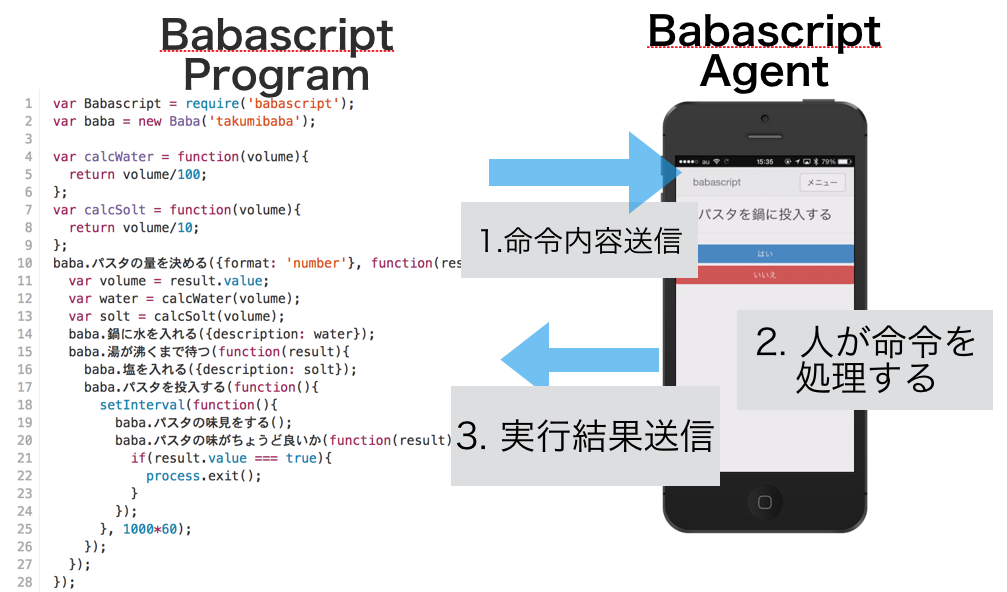
\includegraphics[width=.7\linewidth,bb=0 0 1007 592]{images/overview-using.png}
  \end{center}
  \caption{利用例}
  \label{fig:overview_using}
\end{figure}

以下のような手順で、処理が進む。

\begin{enumerate}
\def\labelenumi{\arabic{enumi}.}
\itemsep1pt\parskip0pt\parsep0pt
\item
  人への指示構文を実行する (Babascript)
\item
  指示内容がNode-Lindaサーバを経由してクライアントへと配信される
  (Node-Linda)
\item
  指示を受け取ったクライアントがユーザに処理を促す (Babascript Agent)
\item
  指示実行者が、指示に従って行動し、その結果を入力する (Babascript
  Agent)
\item
  Node-Lindaサーバを経由して実行元プログラムに入力された処理結果が送信される
  (Node-Linda)
\item
  プログラム側で指定されたコールバック関数が実行される (Babascript
  Agent)
\end{enumerate}

Babascriptプログラミング環境の概要を図\ref{fig:system_image}に示す。

\begin{figure}[htbp]
  \begin{center}
  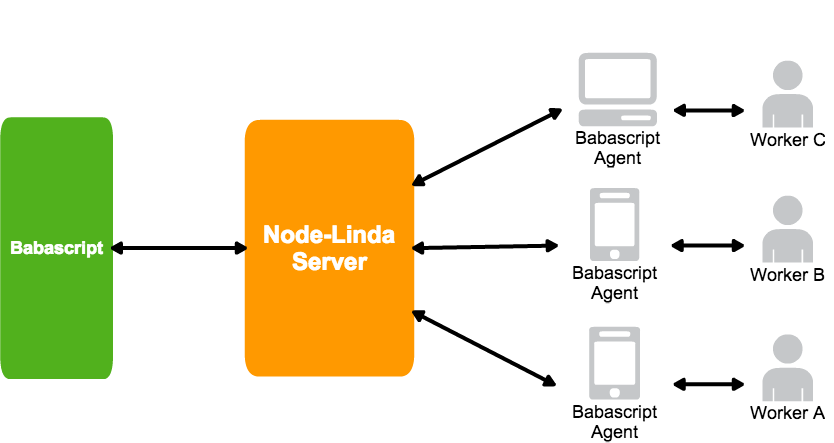
\includegraphics[width=.7\linewidth,bb=0 0 834 443]{images/overview.png}
  \end{center}
  \caption{システム概要}
  \label{fig:system_image}
\end{figure}

\section{Babascript}\label{babascript}

プログラムと人とのインタラクションを実現するためには、プログラムと人間のメッセージングの実現が必要だ。
つまり、プログラム上で人間への指示とその処理結果を受け取る仕組みが必要だ。
そこで、Babascriptという、人間への指示構文を持ったオブジェクト(以下、人間オブジェクト)を宣言できるプログラミングライブラリを実装した。
BabascriptはJavascriptのサーバサイド実行環境であるNode.js及びRubyで実装した。
本論文で示すサンプルソースコードは全てJavascriptで記述したものを掲載する。

\subsection{基本仕様}\label{ux57faux672cux4ed5ux69d8}

Babascriptでは、人間オブジェクトを通して人間とプログラムのメッセージングを行う。
例えば、ソースコード:\ref{code:babascript-sample}のようなプログラムによって、
人間オブジェクトを宣言し、人間へ指示を送ることができる。
人間への指示を送る構文のことを、人間への指示構文と呼ぶ。

\begin{lstlisting}[caption=人への指示構文, label=code:babascript-sample]
// ライブラリの読み込み
var Babascript = require('babascript');
// takumibabaという人間を対象とした人間オブジェクトの宣言
var takumibaba = new Babascript('takumibaba');
// takumibabaに対して"clean_up_your_room"という指示を送る
takumibaba.clean_up_your_room();
\end{lstlisting}

人間オブジェクトは生成時にidを指定する必要がある。
このidを元に、人間への指示構文は指示の配信先を決定する。 例えば、id=baba
に命令を送りたい場合、人オブジェクト宣言時の第一引数にはbabaという文字列を指定する。
指定したidに命令が配信されるため、Babascript
Agent側でも同じidを指定する必要がある。

人間オブジェクトは、構文エラーが存在する場合を除き、
自身に定義されていないメソッドが実行されると、エラーを返さずに人間への指示として解釈する。
そのため、実装されていないメソッド名であれば、あらゆる指示をメソッドとして表現し実行することが可能である。
例えば、「toString」や「call」等のメソッドは、javascriptにおいては多くのオブジェクトが持つメソッドだ。
一方で、「clean\_up\_your\_room」や「bake\_bread」のようなメソッドは定義しない限りは存在しないメソッドである。
Babascriptは、この定義されていないメソッドをエラーとして評価せず、
人への指示構文として評価する(ソースコード:\ref{code:methodmissing-sample})。

\begin{lstlisting}[caption=通常のメソッドと指示構文の例, label=code:methodmissing-sample]
var Babascript = require('babascript');
var baba = new Babascript('takumibaba');

baba.exists_method = function(){return true}

// 上記で定義したメソッド, 人への命令構文ではない
baba.exists_method();
// 既に定義されているメソッド, 人への命令構文ではない
baba.toString();

// 定義されていないメソッド, 人への命令構文として解釈される
baba.clean_up_your_room();
baba.bake_bread();
\end{lstlisting}

オブジェクトに存在しないメソッドが呼び出された時に、特定のメソッドにその処理を委譲するような仕組みは、
プログラミング言語Rubyにおいてはmethodmissingと呼ばれる。
各言語によって名称は異なるが、類似する仕組みが存在する言語は複数存在する。
Babascriptにおいては、node-methodmissing\footnote{https://github.com/geta6/node-methodmissing}というライブラリを利用している。

また、ソースコード
\ref{code:babascript-exec-method}のように、execメソッドを使うことで指示を送ることも可能だ。
execメソッドを利用する場合は、第一引数に命令内容、第二引数にオプション情報、第三引数にコールバック関数を指定する。

\begin{lstlisting}[caption=execメソッドによる指示構文, label=code:babascript-exec-method]
var Babascript = require('babascript');
var takumibaba = new Babascript('takumibaba');

takumibaba.exec("message_to_human", {}, function(result){
  // 処理を記述する
});
\end{lstlisting}

人間への指示として評価されたメソッドは、そのメソッド名と引数を元にしたタスク情報を生成し、タスク配信サーバへと送信する。
この際、メソッド名部分がユーザに命令として提示される文となる。
タスク情報はソースコード\ref{code:task-format}のように構成される。

\begin{lstlisting}[caption=タスク情報の例, label=code:task-format]
var task = {
  name: "takumibaba", // 命令配信先ID
  key: "instruction_body", // 指示内容
  cid: "1420569060.52_0.9777606867719442", // タスクID
  type: "eval", // 命令のタイプ
  option: { // オプション情報
    format: "boolean", // 想定返り値型
  }
}
\end{lstlisting}

メソッド名が自由に設定できるため、内容は指示ではなく、質問のようなものもあり得るが、本研究では統一して指示と呼ぶ。
人への指示構文の第一引数にはオプション情報を指定する。
第二引数には人力処理の実行後に実行するコールバック関数を指定する。
このコールバック関数は、指示に対して何かしらの値が返されたときに実行される。

\subsection{オプション情報の付加}\label{ux30aaux30d7ux30b7ux30e7ux30f3ux60c5ux5831ux306eux4ed8ux52a0}

指示内容以外に送信したい情報があるときには、人への指示構文の引数にオプション情報としてハッシュを与える。
クライアントアプリケーション側でオプション情報を得ることができるため、このオプション情報に応じて
ユーザに提示する画面を変更するといったことが可能である。

オプション情報の例としては、返り値の型情報や、タイムアウト情報などが考えられる。
ソースコード\ref{code:babascript-option}の場合であれば、
返り値の型はstringで、3分後までに返り値を得られなかった時は、
人力処理を止め、第二引数で指定するコールバック関数を実行し、
処理を続行させるといったことがオプション情報として記述されている。

\begin{lstlisting}[caption=オプション情報のサンプルソースコードその1, label=code:babascript-option]
var Babascript = require('babascript');
var baba = new Babascript('takumibaba');

baba.hogefuga({format: 'string', timeout: 1000*60*3}, function(){

});
\end{lstlisting}

また、ソースコード:\ref{code:babascript-option-list}の場合であれば、listで指定した選択肢の中から選んで返り値を返す、といった指定が可能だ。

\begin{lstlisting}[caption=オプション情報のサンプルソースコードその2, label=code:babascript-option-list]
var Babascript = require('babascript');
var takumibaba = new Babascript('takumibaba');

var option = {
  format: 'list'
  list: ['良い', '普通', '悪い']
};
takumibaba.会場の雰囲気はどうですか(option, function(result){
  // 人が処理した結果が引数に格納される。
  // 返り値に応じて処理を分岐させる
  if(result.value == '良い'){
    // ...
  }else if(result.value == '普通'){
    // ...
  }else if(result.value == '悪い'){
    // ...
  }else{
    // ...
  }
});

\end{lstlisting}

特別なオプション情報として、broadcastとinterruptが存在する。
broadcastオプションは、同じ指示を複数のワーカーに同時に配信し、指定した数だけの値を得ることが出来た場合に
コールバック関数を実行するというものだ。
指定した数の値が集まらない場合でも、コールバック関数を実行させることもできる。
タイムアウトオプション等と組み合わせ、5分経ったら得られた値のみを使って処理を継続する、といったことが可能だ。

interruptオプションは、割り込み処理のためのオプションだ。
他の指示が先に送られていても、interruptオプションをつけた指示は優先的に実行されるようキューに割り込んで追加する。
現在実行されているタスクの次のタスクとして登録される。

オプション情報は省略可能である。
省略した場合は、自動的にソースコード:\ref{code:option-default}のようなオブジェクトが代入される。

\begin{lstlisting}[caption=デフォルトのオプション情報, label=code:option-default]
var defaultOption = {
  format: 'boolean'
}
\end{lstlisting}

\subsection{コールバック関数の指定}\label{ux30b3ux30fcux30ebux30d0ux30c3ux30afux95a2ux6570ux306eux6307ux5b9a}

人間への指示構文の最後の引数に関数を代入すると、実行結果を取得した後に代入した関数を実行する。
処理が成功していた場合、この関数に渡される第二引数の中に、実行結果が代入される。
処理が失敗していた場合、第一引数にエラーの内容が代入される(ソースコード:\ref{code:babascript-callback})。

\begin{lstlisting}[caption=コールバック関数の指定, label=code:babascript-callback]
var Babascript = require('babascript');

var baba = new Babascript('takumibaba');
baba.do_callback({format: 'boolean'}, function(result){

});
\end{lstlisting}

また、Promiseによる処理関数の指定も可能である。
人への指示構文実行時、コールバック関数を指定しなかった場合、Promiseオブジェクトがその時点での返り値として返される。
Promiseオブジェクトのthenメソッドに指示に対する処理結果が得られた場合に実行する関数を、
catchメソッドに何かしらのエラーが起きて結果を得られなかった場合に実行する関数を指定する(ソースコード:\ref{code:babascript-promise})。

\begin{lstlisting}[caption=Promiseによる関数指定, label=code:babascript-promise]
var takumibaba = new Babascript("takumibaba");

takumibaba.use_promise({})
.then(function(result){
  // 実行結果が正しく得られた場合の処理を記述する
}).catch(function(error){
  // エラー等で実行結果が得られなかった場合の処理を記述する
});
\end{lstlisting}

\subsection{コマンドラインでの利用}\label{ux30b3ux30deux30f3ux30c9ux30e9ux30a4ux30f3ux3067ux306eux5229ux7528}

Babascriptはコマンドラインツールとしても利用可能だ。
babaコマンドは、ソースコード\ref{code:baba-command}のように利用することができる。
オプションeの直後に指示内容を、オプションnの直後に指示先のIDを指定する。
format情報などを付加したい場合は、オプションoの後に key=value
の形で指定することができる。
コマンドラインで実行することによって、人間による処理をpipeに組み込むといったことも可能になる。

\begin{lstlisting}[caption=Babaコマンド, label=code:baba-command]
% baba -e hogefuga -o format=boolean
\end{lstlisting}

\section{Babascript Agent}\label{babascript-agent}

Babascriptによって人への指示をプログラムに記述し、実行することが可能となったが、
その指示を人に伝え、処理結果を送信するためのアプリケーションが必要となる。
そこで、Babascript Agent というアプリケーションを実装した。 Babascript
Agent
は、Babascriptとの通信を担うサービス部と返り値の入力等を担うインタフェース部から構成される。

\subsection{サービス}\label{ux30b5ux30fcux30d3ux30b9}

サービス部は、主にBabascriptとのやりとり、つまり、命令の受け取りや返り値の送信などを担う。

命令を受け取ると、イベントを発行する

\begin{lstlisting}[caption=Babascript Agent サービス部のソースコード例, label=code:babascript-client-service]
var Client = require('babascript-client');

var client = new Client("takumibaba");
client.on("get_task", function(task){
  // babascriptからの命令を受信した時の挙動を記述
});

client.on("cancel_task", function(task){
  // 命令が何かしらの理由でキャンセルされた時の挙動を記述
});
\end{lstlisting}

何かしらの値を実行結果として返すときは、clientオブジェクトに実装されているretrnValueメソッドを用いる。
ソースコード\ref{code:babascript-client-service-returnvalue}のように、第一引数に結果として返すものを指定する。

\begin{lstlisting}[caption=Babascript Agent 処理結果を返すメソッドの例, label=code:babascript-client-service-returnvalue]
var Client = require('babascript-client')l
var client = new Client('takumibaba');

client.returnValue(true);
client.returnValue(10);
client.returnValue("string");
\end{lstlisting}

実行結果情報として返すデータの例を図\ref{code:return-value-data}に示す。

\begin{lstlisting}[caption=タスク情報, label=code:return-value-data]
value = {
  _task: task, // 元タスクのオブジェクト情報
  value: true, // ワーカーが入力する実行結果
  cid: '1420569060.52_0.9777606867719442', // タスクのID情報
  worker: 'takumibaba', //実行者情報
  options: {},
  type: "return"
}
\end{lstlisting}

命令実行をキャンセルしたい場合は、cancelメソッドを用いる。
cancelメソッドの第一引数に、キャンセルする理由を指定することができる。

\subsection{ユーザインタフェース}\label{ux30e6ux30fcux30b6ux30a4ux30f3ux30bfux30d5ux30a7ux30fcux30b9}

指示のユーザへの提示と、実行結果の入力を担う。
サービス部と独立した実装のため、異なるデバイスや環境上でもインタフェース部を実装するだけでBabascript
Agentの機能を構築可能である。
指示内容と返り値の入力インタフェースをユーザに提示し、返り値の入力を受け付ける。
この際、Babascriptの指示でオプション情報として返り値の型を指定していた場合、
指定した型以外の入力を受け付けないよう実装している。
返り値の型は現在、Boolean, String, Number、Listに対応している。

例として、スマートフォンアプリケーション、slackインタフェースを実装した。

\subsubsection{スマートフォンアプリケーション
プロトタイプ1}\label{ux30b9ux30deux30fcux30c8ux30d5ux30a9ux30f3ux30a2ux30d7ux30eaux30b1ux30fcux30b7ux30e7ux30f3-ux30d7ux30edux30c8ux30bfux30a4ux30d71}

\begin{figure}[htbp]
  \begin{center}
  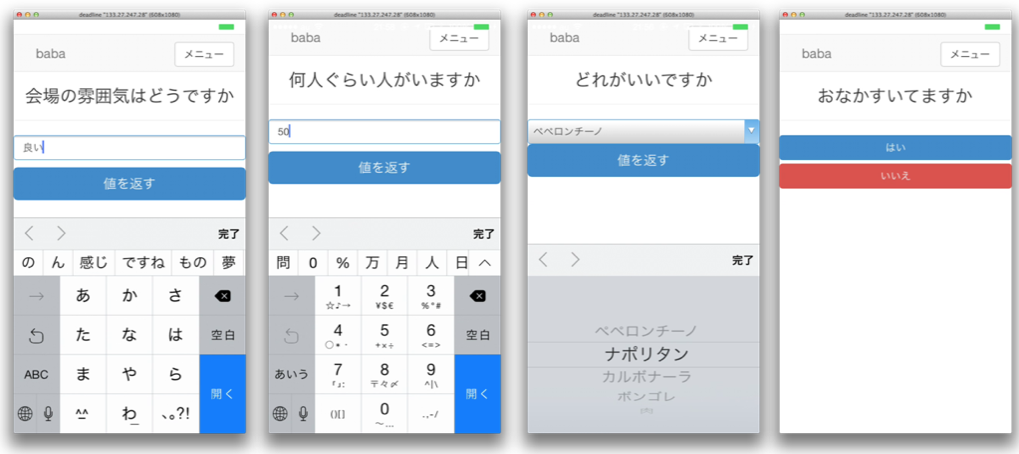
\includegraphics[width=.8\linewidth,bb=0 0 1019 454]{images/interface_list.png}
  \end{center}
  \caption{Babascript Agent Webアプリケーションインタフェース}
  \label{fig:client_format_list}
\end{figure}

インタフェースの例として、スマートフォンアプリケーションとして実装した。
webアプリケーションとして実装し、 Apache
Cordova\footnote{http://cordova.apache.org/}を用いてスマートフォンアプリケーション化した。
android及びiOSアプリケーションとして動作する。
JavascriptのフレームワークにはBackbone.js\footnote{http://backbonejs.org/}とMarionette.js\footnote{http://marionettejs.com/}を利用している。
CSSはSASS\footnote{http://sass-lang.com/}、HTMLはJade\footnote{http://jade-lang.com/}で記述した。
システムは図\ref{fig:client-overview}のように構成される。

\begin{figure}[htbp]
  \begin{center}
  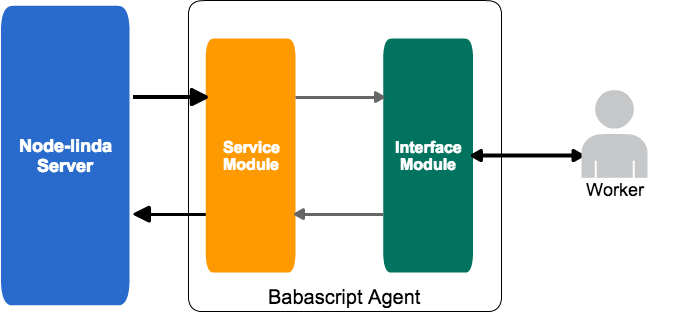
\includegraphics[width=.8\linewidth,bb=0 0 675 312]{images/webapp-system.png}
  \end{center}
  \caption{Babascript Agent webアプリケーションシステム図}
  \label{fig:client-overview}
\end{figure}

Webインタフェースでは、指示内容に応じて提示インタフェースを変化させる実装をしている。
例えば、フォーマットにBooleanを指定していた場合、ユーザには「はい」と「いいえ」の2種類のボタンが提示される。
それぞれのボタンにはtrueとfalseの値が設定されており、ボタンを押すことによって設定された値を返り値としてプログラムに送ることができる。
また、StringとNumberであれば、文字・数字の入力フォームと投稿ボタンが提示され、
投稿ボタンを押した際にフォームに入力されていた内容が返り値としてプログラムに返される。
Listであれば、選択フォームが表示され、リストの中から返り値を選択することができる。
実際に提示されるインタフェースの例を図\ref{fig:client_format_list}に示す。

プログラムからの指示を受け取ると、アプリによる通知を発行し、ユーザに値を返すよう促す(図\ref{fig:client-push-notification})。

\begin{figure}[htbp]
  \begin{center}
  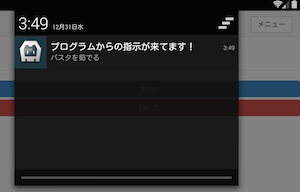
\includegraphics[width=.5\linewidth,bb=0 0 300 192]{images/client-push-notification.png}
  \end{center}
  \caption{Babascript Agent Push通知例}
  \label{fig:client-push-notification}
\end{figure}

指示が実行できない場合には、エラーを値として返すことができる。
例えば、自宅にいるにも関わらず、大学の研究室にいないと出来ないような指示が来た場合には、少なくともその時点では
指示を実行に移すことは出来ない。
エラー処理のインタフェースを図\ref{fig:throw-error}に示す。

\begin{figure}[htbp]
  \begin{center}
  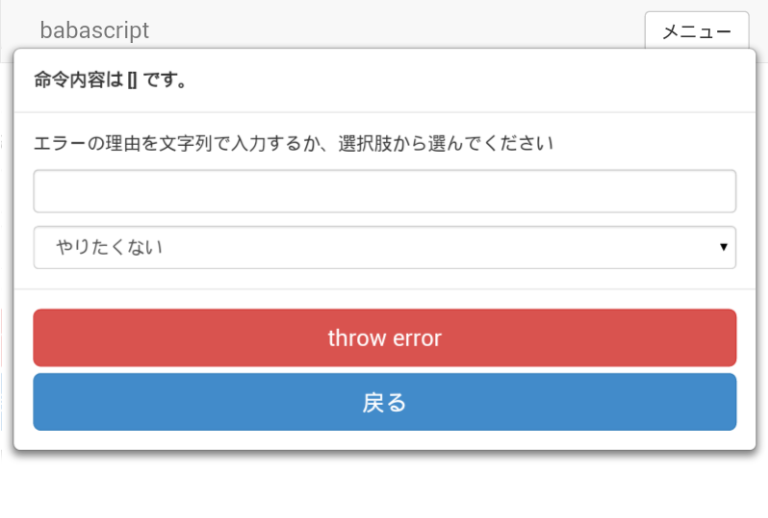
\includegraphics[width=.5\linewidth,bb=0 0 768 518]{images/throw-error.png}
  \end{center}
  \caption{Babascript Agent エラー処理インタフェース}
  \label{fig:throw-error}
\end{figure}

\subsubsection{スマートフォンアプリケーション
プロトタイプ2}\label{ux30b9ux30deux30fcux30c8ux30d5ux30a9ux30f3ux30a2ux30d7ux30eaux30b1ux30fcux30b7ux30e7ux30f3-ux30d7ux30edux30c8ux30bfux30a4ux30d72}

プロトタイプ1では、複数の指示が受けた場合でも一つ一つの指示しか表示できなかった。
人間は実世界で様々な処理を並列で実行していることから、Babascript
Agentにおいても 取得した指示を並列に示すことが望ましい。

そこで、基本的なインタフェースはプロトタイプ1を踏襲し、受けた指示の一覧をTODOリスト風のインタフェースを用いて
ワーカーに提示するアプリケーションを実装した。
こちらのアプリケーションをプロトタイプ2とする。

\subsubsection{チャットボット}\label{ux30c1ux30e3ux30c3ux30c8ux30dcux30c3ux30c8}

チャットサービス上で稼働するボットにBabascript Agentの機能を実装した。
ボットシステムにはHubot\footnote{https://hubot.github.com/}を採用した。
Hubotは様々なチャットサービスに対応しているが、Slackというチャットサービス上において運用している。
このボットシステムは、Heroku\footnote{https://heroku.com}上で稼働している。
チャットボットのシステム図を図\ref{fig:hubot-system}に示す。

\begin{figure}[htbp]
  \begin{center}
  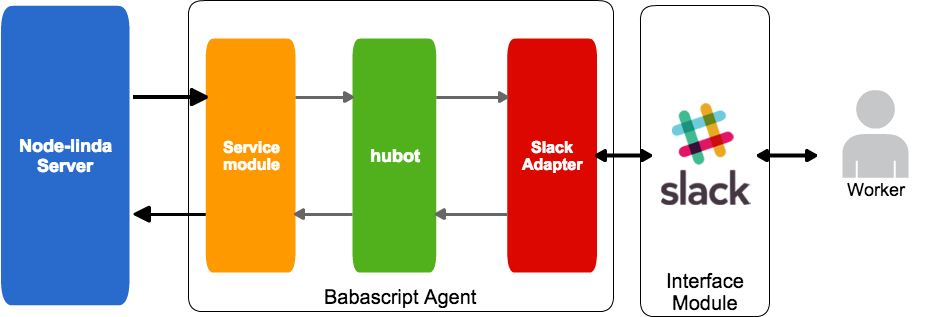
\includegraphics[width=.9\linewidth,bb=0 0 936 312]{images/hubot-system.png}
  \end{center}
  \caption{Hubotシステム図}
  \label{fig:hubot-system}
\end{figure}

チャットボットシステムは、ユーザからのメッセージによる問い合わせに応じて返答を行う。
また、指示を受けた際には、指示内容をリプライとして投稿する。
返答の例を図\ref{fig:babascript_client_slack}に示す。

\begin{figure}[htbp]
  \begin{center}
  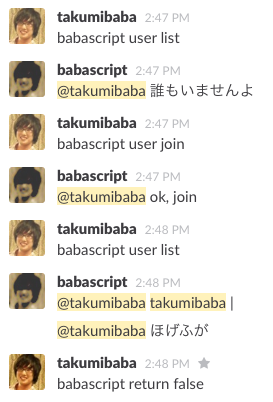
\includegraphics[width=.4\linewidth,bb=0 0 273 402]{images/babascript_client_slack.png}
  \end{center}
  \caption{Babascript Agent Slackインタフェース}
  \label{fig:babascript_client_slack}
\end{figure}

チャットボットインタフェースでは、Webアプリケーションの場合と違い、
提示するインタフェースを返り値の型に応じて変化させるといったことができない。
そのため、ユーザにとっては値を返しにくくなっているが、普段利用しているチャットサービス上で
Babascript Agentの機能を利用できるということは有用なことであると考える。

\section{通信手法}\label{ux901aux4fe1ux624bux6cd5}

BabascriptとBabascript
Agent間の通信のために、仲介サーバとしてNode-Linda\cite{node-linda}を利用する。
通信手法はデバイスごとに利用可能な手法が異なったり限定されるため、交換可能なモジュールとして実装する必要がある。
そこで、分散処理プラットフォームであり、接続方式の追加などを容易に実装可能なNode-Lindaを仲介サーバとして採用した。

Babascript及びBabascript
AgentがNode-Lindaに接続するために実装された通信用のモジュールを、Babascript
Adapterと呼ぶ。
このAdapterを介してNode-Lindaに接続し、情報のやりとりを行う。
本節では、この仲介サーバとして用いるNode-Lindaについて述べた後、2種類のBabascript
Adapterを紹介する。

\subsection{Node-Linda}\label{node-linda}

\subsubsection{概要}\label{ux6982ux8981}

Node-Linda\cite{node-linda}は、分散並列処理のための仕組みであるLinda\cite{linda}をNode.js上に実装したものだ。
Lindaは、タプルスペースという共有メモリを用いてプロセス間でデータの通信を行う並列処理のためのモデルだ。
Node-Lindaでは、Lindaを独自に拡張し、Websocket等を利用して接続できるように実装されている。
接続のためのプログラムさえ記述すれば、あらゆるデバイスがNode-Lindaに接続可能である。
Linda及びNode-Lindaのタプル空間への操作を表\ref{table:tuple-management}にまとめる。

\begin{longtable}[c]{@{}lcc@{}}
\caption{Linda及びNode-Lindaのタプル空間への操作
\label{table:tuple-management}}\tabularnewline
\toprule
操作 & Linda & Node-Linda\tabularnewline
\midrule
\endfirsthead
\toprule
操作 & Linda & Node-Linda\tabularnewline
\midrule
\endhead
書き込み & out & write\tabularnewline
読み込み & rd & read\tabularnewline
読み込みつつ削除 & in & take\tabularnewline
ブロックして読み込み & rdp & -\tabularnewline
ブロックして読み込みつつ削除 & inp & -\tabularnewline
書き込みを読み続ける & - & watch\tabularnewline
\bottomrule
\end{longtable}

各種操作は名称も変更されている。
watch操作と同等の機能は従来のLindaの仕様にはなく、Node-Linda独自の仕様である。
また、Node-Lindaでは非同期処理が前提となっており、ブロック処理は仕様から削除されている。

実世界コンピューティングでの利用を前提としており、様々なセンサーやアクチュエータが接続することが想定される。
Babascriptによる人間の指示や、その実行結果も、センサーやアクチュエータの処理を同じようにNode-Linda上で共有される。
Node-Lindaの各操作は、ソースコード\ref{code:linda-usage}のようなプログラムで実現する。

\begin{lstlisting}[caption=Node-Lindaへの接続方法, label=code:linda-usage]
// Node-Lindaに接続するクライアントの準備
var LindaClient = require('linda').Client;
var socket = require('socket.io-client').connect('http://babascript-linda.herokuapp.com/');
var linda = new LindaClient().connect(socket);

// タプルスペース(共有メモリ空間)の宣言
var tuplespace = linda.tuplespace('babascript');

// タプルスペースへの書き込み
tuplespace.write({"type": "sensor"});

// タプルスペースからデータを読み込む
tuplespace.read({}, function(err, data){
  //
});

// タプルスペースからデータを読み込んで消す
tuplespace.take({}, function(err, data){

});

// タプルスペースへのデータ書き込みを監視する
tuplespace.watch({}, function(err, data){

});

tuplespace.cancel(cid);
\end{lstlisting}

Babascript及びBabascript
Agentは、Adapterを用いてNode-Lindaのタプルスペースの操作を行う。
宣言時に指定するIDを元に使用するタプルスペースを決定する。
通常の指示を書き込むnormalスペース、割り込み処理用に使うinterruptスペースを個別に利用することで、
割り込み処理の優先的に読み込みを実現している。

\subsection{Socket.IO Adapter}\label{socket.io-adapter}

Socket.IO
Adapterは、リアルタイム通信のためのライブラリであるSocket.IO\footnote{http://socket.io/}を用いて
Node-Lindaに接続するためのAdapterだ。
WebsocketもしくはXHR-Pollingによって常にNode-Lindaサーバと通信をし続ける。
全ての処理はSocket.IOによる通信によって実現する。

常時通信している都合上、バッテリー消費の問題が生じたり、デバイスによっては通信を強制的に切断されてしまうことがある。
Socket.IO Adapterは、接続環境が良好な状態での利用が望ましい。

\subsection{PushNotification Adapter}\label{pushnotification-adapter}

PushNotification Adapter は、HTTP
RequestとPushNotificationを用いてNode-Lindaと通信を行うためのAdapterだ。
Cordovaのプラグインとして実装した。 Node-Lindaへのタプル操作はHTTP
Requestの実行によって実現する。
Node-Linda側からAdapter側への通信には、PushNotificationを用いる。 Amazon
AWS
SimpleNotificationService\footnote{http://aws.amazon.com/jp/sns/}を利用し、
PushNotificationを実現している。 PushNotification
Adapterを利用するためには、Node-Linda側でPushNotification
Adapter用のライブラリを読み込む必要がある。

PushNotification
Adapterは、モバイルデバイス等の常時接続が難しいデバイス上で、可能な限りリアルタイムなやりとりを実現するために
実装された通信モジュールだ。
主にAndroidやiPhone等のモバイルデバイスからNode-Lindaと接続する際に利用する。

構成図を図\ref{fig:push-notification-adapter}に示す。

\begin{figure}[htbp]
  \begin{center}
  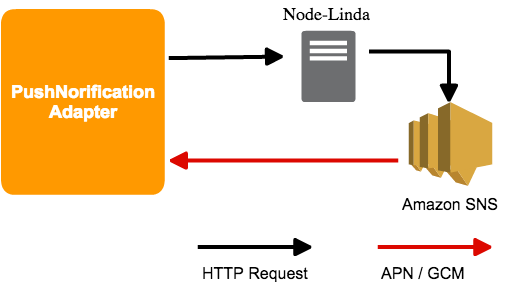
\includegraphics[width=.5\linewidth,bb=0 0 529 303]{images/push-notification-adapter.png}
  \end{center}
  \caption{PushNotification Adapter}
  \label{fig:push-notification-adapter}
\end{figure}

\section{プラグイン機構}\label{ux30d7ux30e9ux30b0ux30a4ux30f3ux6a5fux69cb}

Babascript 及びBabascriptClient
Agentはその機能を拡張するために、プラグイン機構を持つ。

図\ref{code:babascript-plugin}の様に使うことで、Babascript及びBabascript
Agentによってイベントが発生した時に、
それに応じたデータを受け取り、自由に操作することができる。

\begin{lstlisting}[caption=Babascript Plugin, label=code:babascript-plugin]
var Babascript = require('babascript');
var baba = new Babascript('takumibaba');

var Client = require('babascript-client');
var client = new Client('takumibaba');

var logger = require('babascript-plugin-logger');

baba.set logger()
\end{lstlisting}

Babascript及びBabascript Agent
は、表\ref{table:plugin-events}にあるイベントを受け取る。
また、イベントを受け取った際にはイベントに応じたデータを受け取る。

\begin{longtable}[c]{@{}lrr@{}}
\caption{Babascript及びBabascript Agentが発行するイベント一覧
\label{table:plugin-events}}\tabularnewline
\toprule
イベント名 & Babascript & Babascript Agent\tabularnewline
\midrule
\endfirsthead
\toprule
イベント名 & Babascript & Babascript Agent\tabularnewline
\midrule
\endhead
load & ○ & ○\tabularnewline
connect & ○ & ○\tabularnewline
send & ○ & ×\tabularnewline
return\_Value & × & ○\tabularnewline
receive & ○ & ○\tabularnewline
\bottomrule
\end{longtable}

loadイベントは、プラグインが読み込まれた際に発生する。
例えば、設定ファイルの読み込みなどの処理を行う。
connectイベントは、Babascript及びBabascript
AgentがNode-Lindaサーバに接続した際に発生するイベントだ。
sendイベントは、Babascriptによって人間への指示構文が実行された際に発生する。
例えば、指示内容を全てログとして保存したいときなどには、sendイベントと共に受け取るデータを送信するといったことができる。
return\_valueイベントは、Babascript
Agentが指示に対して実行結果を返すときに発生する。
receiveイベントは、Babascript及びBabascript
Agentが何かしらのデータをNode-Lindaサーバから受け取る際に発生する。
指示を送ってから値が帰ってくるまでの時間を計測したいときなどは、このイベントをフックすることで実現可能だ。

プラグイン機構によって、Babascript環境を拡張していくことが容易となる。
例えば、ログを取得してサーバに送信するプラグインや、 Babascript
AgentとBabascript間でのデータの同期を実現するプラグイン、
インセンティブを付与するためのプラグインなどが考えられる。

\section{まとめ}\label{ux307eux3068ux3081}

人間と計算機の処理を融合させたプログラミング環境の具体的な実装や利用方法について述べた。

\chapter{応用例}\label{chap:application}

本章では、Babascriptプログラミング環境によって実現可能と考えられる応用例について述べる

\section{Activity as Code}\label{activity-as-code}

Babascriptプログラミング環境によって、プログラムはコンピュータへの指示系統だけでなく、人間への指示系統を利用できるようになる。

\section{仕事のプログラム化}\label{ux4ed5ux4e8bux306eux30d7ux30edux30b0ux30e9ux30e0ux5316}

人への指示がプログラムとして記述可能になることで、仕事をプログラム化することができると考える。
人の仕事は、例えば、マニュアルのような形で記述されることが多い。
マニュアルはどのように行動すべきかが構造的に記述された手順書であり、「Aという条件の時にはBの処理を実行する」といったことが文章として記述されていることが多い。
コンピュータにとっての手順書であるプログラムとは類似点多く、プログラムに変換可能であると考える。

プログラム化することで、仕事における進行度などの状態をプログラムで管理することができる。
状態を可能な限りプログラムで管理し、経験や知識によって可能な条件判断などもプログラム化することができれば、プログラムに指示されたことのみを実行するだけである程度の仕事を実行できると考える。
指示されたことのみを実行するだけでも良いということは、仕事の引き継ぎなどが最低限となり、人の代替をも容易にする可能性がある。
プログラム経由にすることで、詳細な実行ログや実行状況を把握することも可能である。
仕事の実行量の定量化や、状況監視、状況の可視化などに応用可能であると考える。

また、人同士がコミュニケーションを取ることなく、複数人を協調させるといったことも可能となる。
通常、複数人を協調させるためには、人同士が相談したり、上位の意思決定者が必要となる。
しかし、コミュニケーションはコストのかかるものであり、適切に行われない場合、問題が生じることもある。
意思決定をプログラムに委ねることは、複数人を効率よく協調させることに繋がるとも考えられる。

\section{人の力を利用した実世界プログラミング}\label{ux4ebaux306eux529bux3092ux5229ux7528ux3057ux305fux5b9fux4e16ux754cux30d7ux30edux30b0ux30e9ux30dfux30f3ux30b0}

人をセンサーやアクチュエータとして利用することで、人を使って実世界を操作することが可能となる。
現在のセンサーやアクチュエータでは、実世界に干渉するのには限界がある。
人力処理を組み込むことのできる本提案手法ならば、例えば、コンテキスト情報を伴うようなセンシングであっても、実現可能である。
また、人を汎用的に利用可能なアクチュエータとして利用することもできる。
人をアクチュエータとして利用する、Human as Actuator
と言えるような事例は少ない。
両者を組み合わせることによって、既存の仕組みでは困難であった実世界の操作も可能となると考えられる。

\section{実世界環境の構成管理とテスト}\label{ux5b9fux4e16ux754cux74b0ux5883ux306eux69cbux6210ux7ba1ux7406ux3068ux30c6ux30b9ux30c8}

\section{まとめ}\label{ux307eux3068ux3081}

\chapter{考察}\label{chap:discussion}

本章では、Babascriptプログラミング環境における諸問題や
可能性について述べる。

\section{ユーザインタビュー}\label{ux30e6ux30fcux30b6ux30a4ux30f3ux30bfux30d3ux30e5ux30fc}

実際に試用してもらった上で、インタビューを行った。
インタビューの内容は表\ref{table:interview}の通りである。

\begin{longtable}[c]{@{}lc@{}}
\toprule
& 質問内容\tabularnewline
\midrule
\endhead
問1 &
コンピュータと同じ、処理を実行する立場と言われた時、どう思いますか\tabularnewline
問2 &
自分や他人の感性判断をプログラムに組み込むことについて、どう思いますか\tabularnewline
問3 & 返り値のフォーマット指定は 必要でしたか? \tabularnewline
& 考えの幅が狭まるといったことはありますか? \tabularnewline
& 扱いづらいものはありましたか?\tabularnewline
問4 &
好きなキャラや俳優などからの指示のように見えるインタフェースだった場合、\tabularnewline
& 動きに変化があると思いますか?\tabularnewline
問5 &
命令元の人によって、指示に従うかどうかは変わりますか?\tabularnewline
\bottomrule
\end{longtable}

\section{処理実行単位としての人}\label{ux51e6ux7406ux5b9fux884cux5358ux4f4dux3068ux3057ux3066ux306eux4eba}

本研究において、人間は処理すべきことを指示され実行する存在、コンピュータやセンサーと同じ処理単位としてみなされる。
ユーザインタビューからコンピュータサイエンスに関する研究を行っている大学生及び大学院生に関しては、
特に抵抗がないということがわかったが、コンピュータサイエンスの知見の少ない一般の人にとっては、
コンピュータと同じ存在ということに心理的な拒否感を覚えるといったことが考えられる。
しかし、処理を指示され実行する立場に徹するということは、指示されたことのみに集中していれば良いということであり、
非常に楽なことでもある。
また、コンピュータに出来ることはコンピュータにやらせ、人間は人間が得意なことや人間にしか出来ないようなことを実行する
ことになるため、ワーカーにとっては作業量が減るなどのメリットも存在する。
指示される立場でいるということは、作業を楽にするための一つのアイデアであるとも言える。

また、指示に積極的に従うことによって、今までは実現出来なかった処理が実現したり、全体的な処理の正確性が向上するとすれば
それはワーカー側にとってもメリットであると言える。

\section{プログラム化のメリット}\label{ux30d7ux30edux30b0ux30e9ux30e0ux5316ux306eux30e1ux30eaux30c3ux30c8}

Babascriptプログラミング環境によって様々な処理をプログラム化した際に得られるメリットについて考察する。

まず、プログラムとして記述しておくことによって、コンピュータと一緒に処理を実行していくことができる。
例えば、普通の計算は明らかにコンピュータのほうが得意だ。
人間のインプット等を元にしてコンピュータに計算させれば、高速かつ正確な結果を得られ、人間も計算しなくて良い。
記憶しておくことも、コンピュータのほうが得意だ。
仕事や実世界の状態をコンピュータで管理することによって、時間が経ったりしても正確に情報を引き出すことが出来る。
一方で、あいまいな出来事の処理や感性的な判断を求められる場面、実世界を対象とした処理などは
人間のほうが得意な場面が多い。
人間と計算機やセンサ・アクチュエータを処理に応じて使い分けることによって、より効率的であったり、正確な処理が実現する。

プログラムとして記述することで、様々な情報を取得が容易になる。
Aという処理にかかった時間は、少し前のプログラムの場合は1分であったが、改善することで30秒にすることができた、
というようなことは、解析プログラムを導入することですぐにわかるだろう。
AさんとBさんが同じ処理を実行した場合の実行時間の差などもデータとして取得することが容易となる。
改善の結果が悪ければすぐに元のプログラムに戻す、といったことも、バージョン管理が一般的に行なわれている
プログラムだからこそ、実行しやすい。

また、複数の人間をオーケストレーションし、効率的に動かすといったことも可能になる。
マニュアルなどでは、基本的に一人の人間を対象としている。
しかし、プログラムで記述し、各自に指示を送るようにすれば、複数の人間の指揮も容易であると考えられる。

\section{型指定}\label{ux578bux6307ux5b9a}

Babascriptプログラミング環境においては、人間への指示に返り値の型を指定することができる。
型はBoolean、String、Number、Selectの4種類が存在し、ユーザにはその型に合ったインタフェースが提示される。

型ごとに入力コストが異なるため、指示の実行終了までの時間が変化すると考えられる。
例えば、String型を指定した場合、文字を入力しなくてはならない。
入力する文字を考える時間や文字入力のスピード、文字入力システムの性能等にも左右される。
一方、Boolean型を指定した場合、2択から選んで決定するだけである。
String型とBoolean型では入力コストに差が存在し、他の2つの型においても同様のことが言える。
可能な限り早く値を返して欲しい場合などは、Boolean型を指定することが望ましい。

型を指定されることによって、ユーザ側も入力すべき値がはっきりとし、迷うことがなかったという意見があった。
一方で、String型の場合、指示内容にもよるが入力の自由度が高くなりがちという問題がある。
String型においては、どんな値を入力すれば良いか迷ったり、わからなかったという意見もあった。
これは、どんな値を入力すべきかという例示をすることによって、ある程度解決可能な問題だと考えられる。

\section{処理の実行遅延と実行保証}\label{ux51e6ux7406ux306eux5b9fux884cux9045ux5ef6ux3068ux5b9fux884cux4fddux8a3c}

Babascriptを用いて人に指示を送っても、指示を受け取った人がその場ですぐに処理を実行するとは限らず、
遅延して実行される可能性がある。
指示を受け取るデバイスを見ていないという場合や、指示を受け取っても状況的にすぐに実行できないという場合があると
考えられ、その場合はすぐに指示に対して実行結果を返すことが出来ない。
Babascriptでは、こういった状況に対応するため、非同期実行を前提とした設計にしている。
そのため、人間による処理の実行中はコンピュータ側に他の処理を実行させておくといったことも可能だが、
人間による処理はほぼ確実に全体の処理を遅延させると考えられる。

また、指示を無視するといったことが起きる可能性があり、実行を完全に保証することができない。
上司からの命令などのように、労働上のある程度の強制力がある場合や、
自分自身への指示、家族からの指示などの場合は、無視の可能性は低くなるが、
強制力がない場合は、指示を無視するといったことが起こりうる。
こういった状況においては、何かしらのインセンティブをワーカーに与えることによって実行保障性を確保することが
できると考えられる。

\section{エラーへの対応}\label{ux30a8ux30e9ux30fcux3078ux306eux5bfeux5fdc}

Babascriptからの指示を受け取った時、その指示が想定している状況と、現実の状況が大きく乖離している可能性がある。
場所や時間に依存するような指示の場合等に発生することが予想される。
指示を受け取った時点や場所においては、指定された型では適切な値を返せないといったことが考えられる。
また、無理やり値を返そうとした結果、本来返されるべき値をは異なる値が処理結果として入力されてしまう可能性も存在する。

Babascript
Agentには、実行出来なかった際などに利用するエラー入力用のインタフェースが存在する。
エラーが起きた際、この機能を適切に利用することでプログラム側に通知が可能だ。
現状の実装では、エラーの内容を文字列として入力するか、デフォルトで指定可能な3つの選択肢から選ぶしかない。
エラーの内容を文字列として表現することは難しく、実際に起きたこととは異なるエラーが報告されてしまう可能性もある。
また、ワーカーへの負担も大きくなる。

また、エラーでプログラムが終了した場合、途中から実行しなおすといったことが現状では出来ない。
実世界におけるタスクの多くは、途中で間違っても、その間違いがタスク継続が困難なものでない限り、途中からやり直すといったことが可能だ。
Babascriptで実現するプログラムにおいても、途中からやり直すという機構が求められる。
Turkit\cite{turkit}におけるcrash-and-rerun
programmingの概念のように、途中経過を保存しておくことで、
プログラムの途中から実行し直すという仕組みが実現可能であると考える。
また、途中経過保存によって、どんなタスクがエラーを起こしやすいのかといったことも保存することができ、
ワークフロー改善にも役立つと考えられる。

\section{処理の先送り}\label{ux51e6ux7406ux306eux5148ux9001ux308a}

プログラムから指示を受け取った時、今でなくても後でなら処理できるという状況が存在する。
しかし、そのまま指示を放置していては、タイムアウト処理等によって指示が撤回されてしまったり、
他の処理が遅延してしまう可能性が高い。
処理の先送りをプログラムに通知しておき、またあとで指示を通知し直すなどの仕組みを用意する必要がある。

これは、Babascirpt
Agent側にも非同期的に指示を通知するインタフェースが必要となる、ということである。
現状では、Babascript Agentは完全に同期的な挙動をする。
先送りした指示や現時点でキューに溜まっている指示などをリスト型のインタフェースで表示しておき、
実行する処理を選べるような設計をすることで、Babascript
Agent側で処理の先送りを実現可能である。

\section{割り込み処理}\label{ux5272ux308aux8fbcux307fux51e6ux7406}

コンピュータが多くの割り込み処理を行っているのと同じように、
様々な指示が送られる中で、人間に対しても、指示を割り込みできるような仕組みが求められる。
例えば、現実においても、割り込み処理は多くなされている。
料理をしてる時に、鍋が吹きこぼれそうだったら、他の処理を中断してでも鍋から吹きこぼれないような処理を行う。

このような割り込み処理を、Babascriptでは、人間の指示構文実行時のオプション情報として
特別なフラグを立てることで実現させている。
人間への指示は、Node-Linda上にキュー形式で保存されているが、
この指示のキューを通常タスクと優先タスクで分けて保存している。
優先タスクキューに指示が入ってる場合は、こちらのキューから優先して指示を取得する。

割り込み処理に関しては、Babascript Agent 側の工夫が非常に重要になる。
実世界における割り込み処理の通知は非常にわかりやすい。
鍋が吹きこぼれそうなら、視覚的にわかりやすく通知が行なわれ、
機械がエラーで止まれば、エラー音による通知が行われる。 Babascript
Agentにおいても、割り込み処理が来た際にはわかりやすく通知することが望ましい。
現状では、高度な工夫は実現できていない。
割り込み処理であるということを明示的にし、割り込んだ処理をすぐに行うように
誘導させられるようにインタフェースを再実装する必要がある。

\section{命令の抽象度設計の必要性}\label{ux547dux4ee4ux306eux62bdux8c61ux5ea6ux8a2dux8a08ux306eux5fc5ux8981ux6027}

Babascriptでは、人への指示構文の記述には制限がない。
そのため、命令の抽象度はプログラマの指示記述能力に依存する。
抽象度が高すぎる指示内容にしてしまうと、ワーカーにとって実行内容が理解しづらくなってしまう。
結果として、想定外の処理が実行されたり、意図しない処理結果を返される可能性が存在する。
人間は柔軟な解釈が可能なため、ある程度は補正可能だと考えられるが、補正が不可能なほど抽象的な
指示内容の場合、問題が発生する。

具体的過ぎる命令は、全体の処理内容にもよるが、プログラム自体が冗長となり得る。
プログラムとワーカーの間のやりとりが増え、通信や待機時間、入力時間などによって処理全体が遅延すると考えられる。
また、ワーカーにとっても、やりとりが増えることで、入力の手間が増え、負担増に繋がる。

指示ごとに異なると考えられるが、命令文は適切な抽象度に設計しなくてはならない。

\section{異なる種類の指示の複数同時実行}\label{ux7570ux306aux308bux7a2eux985eux306eux6307ux793aux306eux8907ux6570ux540cux6642ux5b9fux884c}

複数のプログラムから同時に一人の人間に複数の関係のない指示が実行される可能性がある。
例えば、料理プログラムと掃除プログラムが同時に実行された場合、
鍋で何かを煮ている途中に、「洗剤を投入する」といった指示がなされるといったことが考えられる。

現実世界で同じようなことが起きても、人間は指示を分類し、別スレッドで動作させることで問題を回避する。
Babascript Agent
Webアプリケーションプロトタイプ2では、指示を並列に表示させ、
人間側が自分で記憶を元に分類しておくことでこの問題を部分的に解決している。
しかし、類似した指示が来た場合、混同してしまう可能性がある。
どのプログラムからの指示なのかを区別し、
分類し提示するインタフェースを実装することで解決可能と考えられる。

\section{Babascript
Agentへのキャラクター性の付与}\label{babascript-agentux3078ux306eux30adux30e3ux30e9ux30afux30bfux30fcux6027ux306eux4ed8ux4e0e}

Babascript Agentは、一種のソフトウェアエージェントである。 Babascript
Agentを用いた、人とプログラムのコミュニケーションは
ヒューマンエージェントインタラクションであると言える。
ヒューマンエージェントインタラクションとは、
人間とソフトウェアエージェントやロボット間のインタラクション
設計に関する研究分野である。
ヒューマンエージェントインタラクション研究の分野においては、ソフトウェアエージェントやロボットに対して
擬人化手法を適応させることによって、エージェントをより人間らしく見せたり、コミュニケーションを取りやすく
するといった研究がなされている。

擬人化エージェントがもたらす効果については、村上らによる研究\cite{murakami}では、エージェントに人間関係を適応させた実験を行っている。
村上らの実験では、研究室の教官と学生の関係を利用し、教授の顔を模したキャラクターと関係のないキャラクター、両者からの
依頼に対して学生の行動が変化するかどうかを観察した。
実験の結果、教官キャラクターのほうがより依頼を受理されやすいという結果がわかった。
この実験結果から、エージェントに人間関係、特に上司などを模したキャラクターをユーザに提示することである程度、
依頼に対してポジティブにとらえてもらうことが可能だと考えられる。

上記の実験結果は、Babascript Agentにも応用可能である。 Babascript
Agentにキャラクター性を持たせ、そのキャラクターとコミュニケーションを取っているかのように見せる
インタフェースを開発すれば、指示が受理されやすくなる可能性が存在する。
また、キャラクター性の付与によって、プログラムからの指示であるという印象が薄れ、
指示に対する拒否感も薄れるといったことが考えられる。

\section{今後の展望}\label{ux4ecaux5f8cux306eux5c55ux671b}

今後は、本章で述べた問題点についての改善を主に行う。
割り込み処理や処理の先送りは特にBabascript Agent側の改良が必要である。
エラー処理に関する問題も、非常に興味深く、利便性を上げるために解決が必須である。
また、Babascript
Agentへのキャラクター性付与による人間の心理面の変化など、実験の上、その効果を検証したい。

\chapter{関連研究}\label{chap:related}

本章では、本研究に関連する研究を分類し、それらの特徴や本研究との関連性について示す。

\newpage

\section{HumanComputation}\label{humancomputation}

コンピュータの計算能力だけでは解決できない問題を、人間の処理能力を計算資源として利用することによって解決する手法は、
ヒューマンコンピュテーション\cite{humancomputation}と呼ばれ、様々な研究が行なわれている。
現在のコンピュータの技術では、パターン認識など、高い精度で処理することが困難な分野が存在する。
こういった分野において、人間という柔軟な思考能力を持つ資源をコンピュータの代替として用いることで、
より高い精度の処理を実現することが可能である。

\paragraph{reCAPTCHA}\label{recaptcha}

\mbox{}

コンピュータの文字認識能力では処理しきれない文字の認識を人間に実行させるreCAPTCHA\cite{recaptcha}は、
人間かコンピュータかを判別するために文字認識をさせるCAPTCHA\cite{captcha}を応用したものだ。
reCAPTCHAでは、人間に2種類の単語が書かれた画像が提示され、書かれている文字を入力させる。
片方の画像は文字認識がされており、書かれている内容がわかっている。
もう片方は文字認識されていないもので、人間に認識させることでその答えを学習させる。
人間かコンピュータかの判別を行いつつ、未認識の文字の認識作業に協力してもらうことができる仕組みである。

\begin{figure}[htbp]
  \begin{center}
  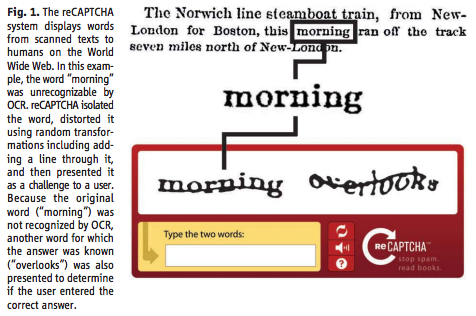
\includegraphics[width=.5\linewidth,bb=0 0 476 316]{images/recaptcha.png}
  \end{center}
  \caption{人間がコンピュータの代わりに文字認識をするシステム reCAPTCHA}
  \label{fig:recaptcha}
\end{figure}

\paragraph{Duolingo}\label{duolingo}

\mbox{}

Duolingo\cite{duolingo}は、ユーザの言語学習における翻訳作業を利用して、ウェブサイトや文書の翻訳を行うアプリケーションだ。
言語翻訳のための計算資源として人間を利用している。
言語学習自体もゲーミフィケーションを活用したものとなっており、翻訳作業しているということは隠蔽された形で語学学習できる。

\paragraph{Vizwiz}\label{vizwiz}

\mbox{}

人間を物体認識エンジンとして利用することのできるアプリケーションが、Vizwiz\cite{vizwiz}だ。
認識したい物体をカメラで撮影し、質問内容などを録音して送ると、インターネットを介して人に処理を依頼し、結果を得ることが出来る。

\paragraph{Soylent}\label{soylent}

\mbox{}

Soylent\cite{soylent}は、文章の校正をインターネットを介した人間の力を利用して行うソフトウェアだ。
文章を意味が通じる状態を維持して短くしたり、文法的に正しくても意味の通じない文章を意味が通じるようにする作業は、人間のほうが得意である。

\paragraph{CrowdDB}\label{crowddb}

\mbox{}

計算機だけでは処理が困難なクエリに対して、人間を用いることで返答可能にする仕組みとして、
CrowdDB\cite{crowddb}が提案されている。
CrowdSQLという、SQLを拡張したものが記述言語として使われる。

\paragraph{Realitime-Captioning}\label{realitime-captioning}

\mbox{}

Laseckiら\cite{realtime-captioning}は、スピーチの動画等にリアルタイムでキャプションを付与するためのエンジンとして
人間を利用する手法を提案している。
通常、リアルタイムのキャプション付けに熟練した人間でないと出来なかった作業を、
非熟練の人間に複数人用意し、スピーチ動画を少しづつキャプション付けさせ、最終的に結合することで実現させている。

\section{CrowdSourcing}\label{crowdsourcing}

インターネットを介して不特定多数の人間に仕事を依頼する仕組みはクラウドソーシングと呼ばれ、近年注目を浴びている。
クラウドソーシングとは、業務の一部を外部に委託することを示すアウトソーシングという言葉を改変した造語である\cite{riseofcrowdsourcing}。
インターネットを介した不特定多数の人間たち(crowd)に仕事をアウトソースすることから、crowdsourcingと呼ぶ。
非常に安価で、かつ、必要な人員をすぐに確保して仕事依頼が可能である。
近年では、Amazon Mechanical
Turk\cite{amt}(以降MTurk)等のクラウドソーシングプラットフォームが登場してきたことによって
多くの利用例が生まれている。
クラウドソーシング分野の研究では、ヒューマンコンピュテーションの概念をクラウドソーシングを利用することで
大規模な人力処理を実現させている。

本節では、クラウドソーシングをより便利に扱えるようにする研究について紹介する。

\paragraph{Turkit}\label{turkit}

\mbox{}

Littleらは、MTurkをプログラムから簡単に利用するためのツールキットであるTurkit\cite{turkit}を提案している。
Turkitでは、通常のプログラミング記法と同じような記法でタスクをクラウドソーシングすることができる(図\ref{fig:turkit})。
また、クラウドソーシングによる処理結果の保存をしておくことで、その後の処理でプログラム実行に失敗しても
再度クラウドソーシングに処理依頼をするのではなく、保存済みの結果を元にプログラムを再度実行できるような仕組み
であるthe crash-and-return プログラミングモデルを提唱している。
可能な限り従来のプログラミング記法を崩さずに人力処理を組み込むことを目的としており、本研究と類似している。
本研究は、クラウドソーシング処理を前提としておらず、特定の個人に対する指示を実現するものである。
Turkitでは特定個人に対する処理依頼を記述することはできない。

\begin{figure}[htbp]
  \begin{center}
  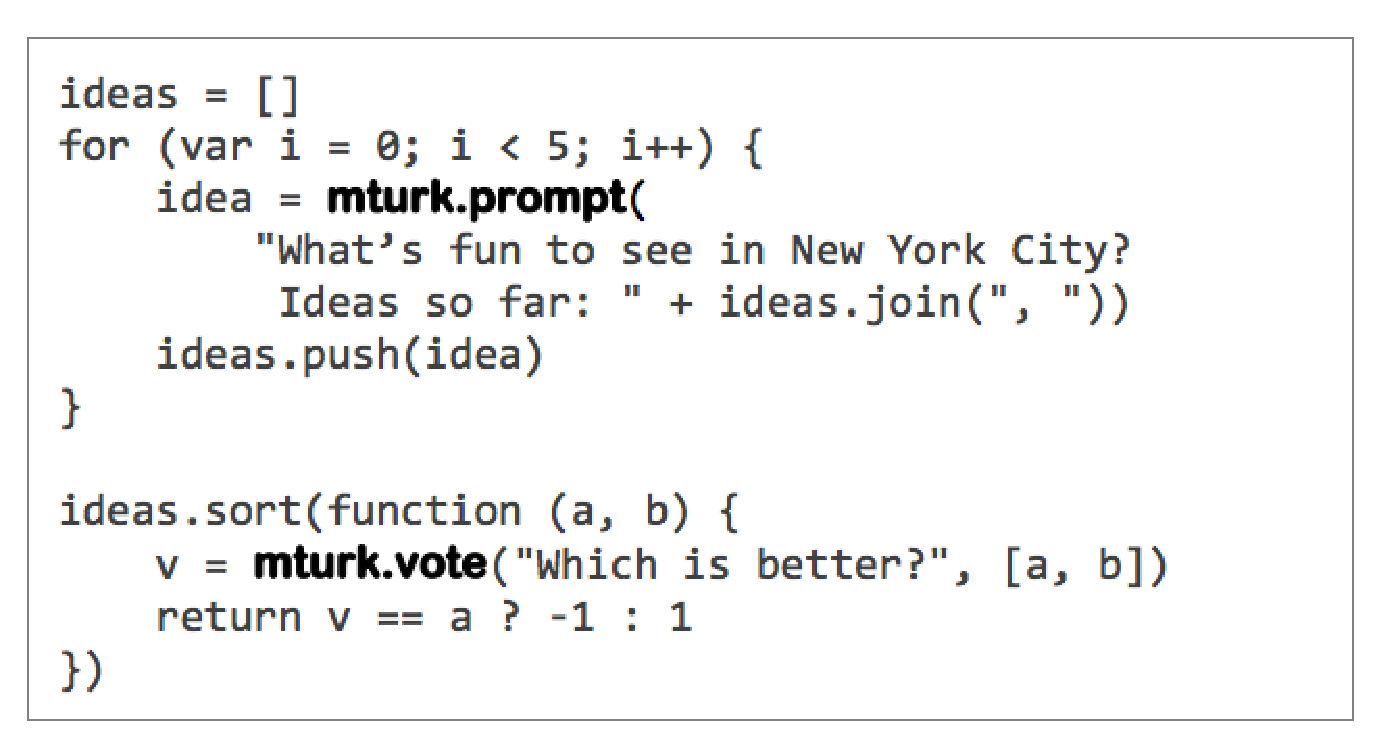
\includegraphics[width=.6\linewidth]{images/turkit.eps}
  \end{center}
  \caption{Turkit}
  \label{fig:turkit}
\end{figure}

\paragraph{Automan}\label{automan}

\mbox{}

Barowyらは、Automanというプログラミング言語Scala上で動作するDomain
Specific Languageを提案した\cite{automan}。
可能な限り通常のプログラミング記法を崩さずにクラウドソーシングを活用した人力処理を組み込むことを目的としており、
クラウドソーシングによる計算とコンピュータによる計算を統合したCrowdProgrammingを提案している。
また、回答の品質管理機能やタスクのスケジューリング、予算の配分等に関する機能を持つ。
本研究における目的は人間と計算機への指示を融合させたプログラミングを実現させることとなっており、類似している。

\begin{figure}[htbp]
  \begin{center}
  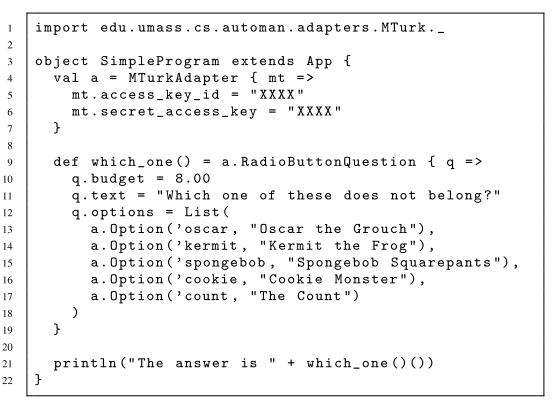
\includegraphics[width=.6\linewidth,bb=0 0 552 404]{images/automan.png}
  \end{center}
  \caption{Automan}
  \label{fig:automan}
\end{figure}

\paragraph{Cylog / Crowd4U}\label{cylog-crowd4u}

\mbox{}

Morishimaらは、人間と計算機の知の融合を目指した環境として、Cylog\cite{cylog}というDatalog\footnote{http://docs.racket-lang.org/datalog/}に類似した構文規則を持った
プログラミング言語と、その実行基盤であるCrowd4U\footnote{http://crowd4u.org/}を提案している。
Cylogでは人間を合理的に動くデータソースとして定義し、プログラム上で利用する。
類似した文法で人間と計算機の双方への命令を記述できる。
また、Crowd4Uという専用の実行基盤も実装しているなど、本研究との類似性が高い。

本研究では、クラウドソーシングそのものを利用していない。
また、Cylogでは人間をデータソースとして利用するが、本研究では人間はデータソースに限らず、汎用な処理の実行対象として利用する。

\paragraph{CrowdForge}\label{crowdforge}

\mbox{}

Kitturら\cite{crowdforge}は、複雑な仕事をクラウドソーシング上で実現するための仕組みとして
CrowdForgeというシステムを提案している。
CrowdForgeはMapReduceの仕組みをクラウドソーシングに適応させた。

\begin{figure}[htbp]
  \begin{center}
  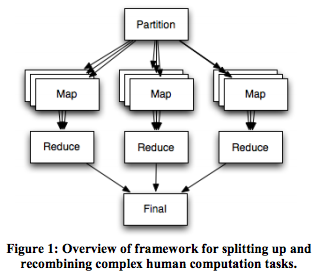
\includegraphics[width=.6\linewidth,bb=0 0 318 276]{images/crowdforge.png}
  \end{center}
  \caption{CrowdForge}
  \label{fig:crowdforge}
\end{figure}

\paragraph{Community Based
Crowdsourcing}\label{community-based-crowdsourcing}

\mbox{}

クラウドワーカーを何かの要素ごとにまとめたグループをコミュニティと呼び、
そのコミュニティの人たち及びコミュニティを横断したクラウドソーシングの仕組みについて提案している\cite{community-based-crowdsourcing}。
コミュニティは動的に変更することができるなど、柔軟にその構成を変化させることが出来る。

\section{Social Computing}\label{social-computing}

コンピュータ・ネットワーク上における群衆の様々な行動や叡智をフィードバックデータとして
システムに組み込み活用していくことはソーシャルコンピューティングと呼ばれている。
例えば、群衆による叡智が集められた情報をまとめるためのプラットフォームとしてはWiki\cite{wiki-way}が存在する。
Wikiの具体的なシステム例で有名なWebサービスがWikipedia\footnote{http://wikipedia.org}である。
また、人々が作るwebページのリンク関係からWebページの重要度を算出するアルゴリズムとしては、PageRank\cite{pagerank}が存在する。
PageRankは検索サービスのGoogle\footnote{https://google.com}で利用されている。
群衆の嗜好情報等を蓄積し、個人間の嗜好等の類似度から情報の推薦等を行う手法は協調フィルタリングと呼ばれる\cite{collaborative-filtering}。

このように、インターネットを介した群衆の叡智を利用してシステムもしくはそのコンテンツを改良していく仕組みは
非常に有用で、多くのWebサービスに活かされている。
次に、特に本研究と関連するソーシャルコンピューティングの事例を紹介する。

\paragraph{The Dog Programming
Language}\label{the-dog-programming-language}

\mbox{}

Webアプリケーションにおけるユーザとのインタラクションの記述に特化したプログラミング言語として、Dog\cite{dog}が提唱されている。
本研究も、人とのインタラクションの記述に特化したものであり、類似している。
DogはWebアプリケーションの実装時によくあるユーザとのインタラクションの記述に特化したものであるが、
本研究は人間を計算資源として様々な処理の実行指示を送るための仕組みである。

\begin{figure}[htbp]
  \begin{center}
  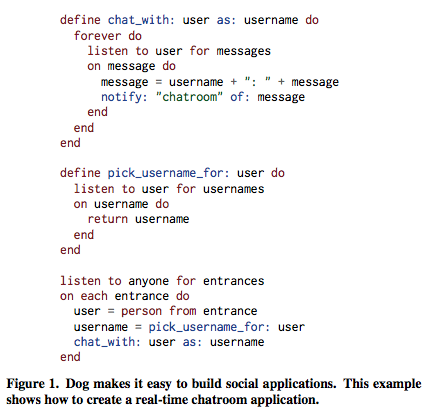
\includegraphics[width=.6\linewidth,bb=0 0 426 414]{images/dog.png}
  \end{center}
  \caption{The Dog Programming Language}
  \label{fig:dog}
\end{figure}

\paragraph{The Jabberwocky Programming
Environmets}\label{the-jabberwocky-programming-environmets}

\mbox{}

Ahmadらは、Jabberwockyというソーシャルコンピューティングのためのプログラミング環境を提案している\cite{jabberwocky}。
Jabberwockyは、様々なクラウドソーシングプラットフォームを統合して管理できるDormouseと、
Dormousとのインタラクションに特化したDog,
MapReduceを人力処理に適応したManReduceから構成される。

\paragraph{Personal APIs As an Enabler for Designing and Implementing
People As Social
Machines}\label{personal-apis-as-an-enabler-for-designing-and-implementing-people-as-social-machines}

\mbox{}

Buregioらは、Social
Machine\cite{social-machines}という研究分野について整理し、その具体的な例として
Personal APIs\cite{personal-api}を提唱している。 Social
Machineは、SocialSoftwareとPeople as Computational Units、Software as
Sociable Entitiesの 3つの領域が重なり合った研究領域である。
この領域において、人間にAPIを付与し、情報にアクセス可能にするという仕組みが、Personal
APIsという概念である。
このAPIを通して、例えばカレンダー情報等にアクセスする。
実装はなく、概念の提唱にとどまっている。

\section{Human as Sensor}\label{human-as-sensor}

人間をセンサー代わりにしたり、人間が持つスマートフォン等のデバイスのセンサーを利用する手法はHuman
as Sensorや参加型センシング\cite{participatory-sensing}と呼ばれる。
ユビキタスコンピューティング\cite{weiser1991computer}などの研究分野において、こういった手法が多く研究されている。
その事例を以下に紹介する。

\paragraph{PRISM}\label{prism}

\mbox{}

Dasらは、PRISM\cite{prism}というスマートフォンを利用した参加型センシング実現のためのプラットフォームを提案している。
参加型センシングをより現実的に実行可能にするためには、セキュリティやスケーラビリティのバランスが取れた
より使いやすいプラットフォームが必要とされているとし、そのためのプラットフォームとしてPRISMを提案している。

\begin{figure}[htbp]
  \begin{center}
  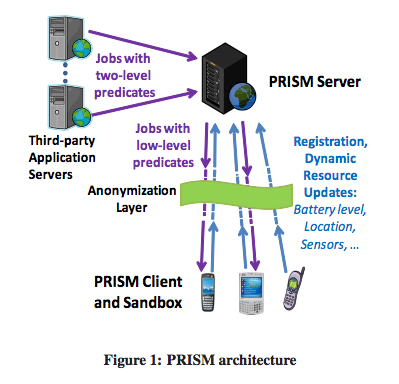
\includegraphics[width=.6\linewidth,bb=0 0 399 384]{images/prism.png}
  \end{center}
  \caption{PRISM: Platform for Remote Sensing using Smartphones}
  \label{fig:prism}
\end{figure}

\paragraph{Moboq}\label{moboq}

\mbox{}

Liuらは、リアルタイムな位置情報ベースQ\&AサービスのMoboQを提案している\cite{moboq}。
マイクロブログサービスを利用したシステムであり、指定した場所にいる人間を対象とした参加型センシングシステムとなっている。

\section{Human as Actuator}\label{human-as-actuator}

アクチュエータ技術は進歩しているが、未だに人間のような汎用的に実世界に干渉できる装置はない。
そこで、人間をアクチュエータの代替として利用し動かす、つまり、人間とロボットの協調によって問題を解決しようという研究がある。

\paragraph{HapticTurk}\label{hapticturk}

\mbox{}

Hapticturk\cite{hapticturk}は、人間をモーションプラットフォームのモーターやメカニカル機構の代わりに使うことによって、
モーションプラットフォームの動きを再現するというものだ。
人間への動きの指示はスマートフォンなどを経由して行なわれる。
人間をアクチュエータの代わりに利用するといった点において、本研究と類似している。
本研究では、その用途をアクチュエータに限ったものではない。
また、プログラム上で汎用的に利用可能である。
Hapticturkでは、ゲームにその用途を限定している。

\begin{figure}[htbp]
  \begin{center}
  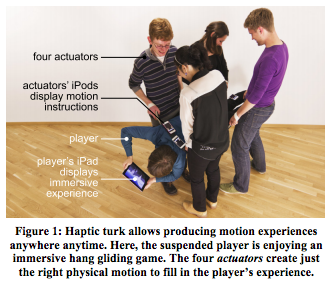
\includegraphics[width=.6\linewidth,bb=0 0 332 281]{images/hapticturk.png}
  \end{center}
  \caption{Hapticturk}
  \label{fig:hapticturk}
\end{figure}

\paragraph{Sharedo}\label{sharedo}

\mbox{}

加藤ら\cite{sharedo}は、ロボットや様々なソフトウェアエージェントと人間のタスクを
同列に記述可能なタスク共有アプリケーションを提案している。
タスクの実行主体は人間でもコンピュータでも良いようになっており、人間とコンピュータは処理実行対象として
同等となっている。 また、Human
Actuation等の概念についても論文内において触れられている。
処理実行対象を選ばないという点において、本研究と類似している。

\begin{figure}[htbp]
  \begin{center}
  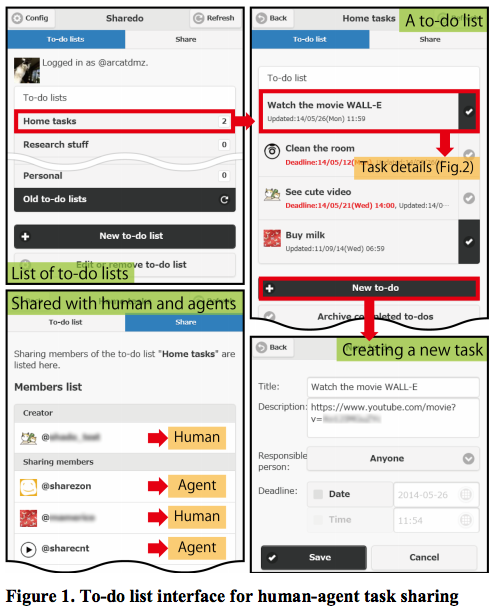
\includegraphics[width=.5\linewidth,bb=0 0 497 611]{images/sharedo.png}
  \end{center}
  \caption{Sharedo}
  \label{fig:sharedo}
\end{figure}

\paragraph{グラフィカルデータフローによる調理レシピプログラミング言語の提案}\label{ux30b0ux30e9ux30d5ux30a3ux30abux30ebux30c7ux30fcux30bfux30d5ux30edux30fcux306bux3088ux308bux8abfux7406ux30ecux30b7ux30d4ux30d7ux30edux30b0ux30e9ux30dfux30f3ux30b0ux8a00ux8a9eux306eux63d0ux6848}

\mbox{}

吉川らは調理レシピを記述するためのデータフロープログラミング言語を提案している\cite{recipe-programming}。
料理レシピをグラフィカルなデータフローで記述する。
料理レシピプログラムは、コンピュータではなく人間が実行するためのものである。
本研究のように、人間がプログラムからの指示を実行することを前提としたものとなっている。

\paragraph{Cooky}\label{cooky}

\mbox{}

Sugiuraらは、人間とロボットが協調して調理をするシステムCooky\cite{cooky}を提案している。
料理支援ロボットと人とロボットが共有可能な調理器具やキッチン、調理手順を記述するシステムから成り立っている。
調理手順記述システムでは、人間とロボット双方の処理を分けて記述することができる。
人間とロボットが協調して作業を実行していくモデルは、本研究が実現したい目標とも似ている。
また、人間の作業タイミング時に人間に作業内容を提示する仕組みなど類似する点は多い。

\begin{figure}[htbp]
  \begin{center}
  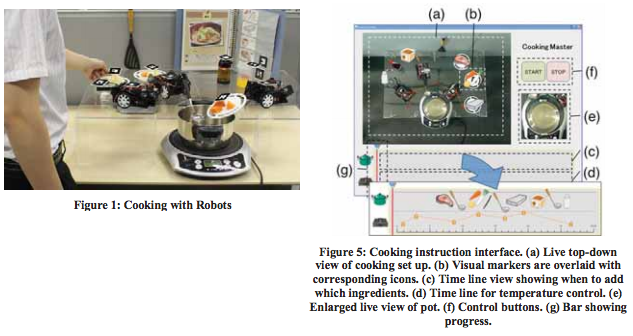
\includegraphics[width=.6\linewidth,bb=0 0 633 336]{images/cooky.png}
  \end{center}
  \caption{Cooky}
  \label{fig:cooky}
\end{figure}

\section{Workflow Programming}\label{workflow-programming}

仕事などにおけるプロセスを文書などによってパターンとして規定し、検証や再利用しやすくするためのものとして
ワークフローというものがある。
このワークフローを構築するための仕組みが複数存在する。

YAWL\cite{yawl}は、ワークフローやビジネス・プロセスを記述するためのワークフロー記述言語だ。
類似のものとしては、XPDL(XML Process Definition
Language)\cite{xpdl}が存在する。
これらのワークフロー記述言語を実行するワークフローエンジンと呼ばれるソフトウェアも多く存在する。
ワークフロー記述言語は、ワークフローを記述するものである。
プログラムによる処理を記述することはできない。

また、X-point\footnote{https://www.atled.jp/xpoint/}や
questetra\footnote{http://www.questetra.com/ja/}といった
ワークフロー記述・実行のためのWebサービスも存在する。

\section{まとめ}\label{ux307eux3068ux3081}

人間の力を積極的に利用し様々な処理に活かすことは、既存研究からも有用であると考えられる。
その多くはコンピュータでは実現が難しい人間の柔軟な演算能力を用いるものである。


\chapter{結論}\label{chap:conclusion}

\section{おわりに}\label{ux304aux308fux308aux306b}

本論文でやったことをまとめる。

今後の展望について語る


\begin{acknowledgment}

修士課程の2年間、研究をご指導いただいてきた慶應義塾大学環境情報学部の増井俊之教授に深く感謝致します。
また、本研究の副査としてご意見、ご助言を頂きました徳田教授、田中准教授に感謝致します。

インタラクションデザインプロジェクトに在籍し、メンバーたちと多くの議論をすることができました。
橋本翔さんには、

shokaiさん
同期 臼杵・nekobato・ゆうくん
後輩 nikezono・keroxp,増井研学部一同
getaさん, 秋山さんとか

本研究は、独立行政法人情報処理推進機構 2013年度未踏IT人材発掘・育成事業の支援を受けました。
未踏事業の中でプロジェクトマネージャーとして多くの助言を頂きました大阪大学の石黒浩教授に感謝致します。
未踏事業の同期のメンバーとは、研究を進めていく上で重要となった議論を多く交わすことができました。
また、多くのOBの方々にもアドバイスを頂きました。感謝致します。

お世話になったひとたち

テンプレートさんきゅー、kurokobo and ymrl

\end{acknowledgment}
  % 謝辞。要独自コマンド、include先参照のこと

\chapter*{本研究に関する発表}
\label{chap:publications}

\section*{学会}

\begin{itemize}
\itemsep1pt\parskip0pt\parsep0pt
\item
  \textbf{馬場匠見} , 橋本翔, 増井俊之
  実世界プログラミングのための分散人力処理環境,
  第6回データ工学と情報マネジメントに関するフォーラム(DEIM2014)
  口頭発表(査読なし)\\ \textbf{{[}学生プレゼンテーション賞{]}}
\item
  \textbf{馬場匠見} , 橋本翔, 増井俊之 Babascript:
  人とコンピュータの協調による処理実行環境,
  第22回インタラクティブシステムとソフトウェアに関するワークショップ(WISS2014),
  口頭発表(査読あり)
\end{itemize}

\section*{展示会}

\begin{itemize}
\itemsep1pt\parskip0pt\parsep0pt
\item
  SFC OpenResearchForum2013 (2013年11月22日〜23日
  東京ミッドタウンホール \&
  カンファレンス、主催:慶應義塾大学SFC研究所)
\end{itemize}

\section*{その他}

\begin{itemize}
\itemsep1pt\parskip0pt\parsep0pt
\item
  独立行政法人情報処理推進機構 2013年度未踏IT人材発掘・育成事業\\
  テーマ名: 実世界プログラミングのための分散人力処理環境の開発
\end{itemize}


\begin{bib}[100]
% BibTeXを使う場合
\bibliography{main}

%\begin{thebibliography}{#1}
%
%  \bibitem{参照用名称}
%    著者名:
%    \newblock 文献名,
%    \newblock 書誌情報,出版年.
%
% \bibitem{hoge09}
%   ほげ山太郎,ほげ山次郎:
%   \newblock ほげほげ理論のHCI分野への応用,
%   \newblock ほげほげ学会論文誌,Vol.31,No.3,pp.194-201,2009.
%
% \bibitem{hoge08}
%   Taro Hogeyama, Jiro Hogeyama:
%   \newblock The Theory of Hoge,
%   \newblock {\it The Proceedings of The Hoge Society}, 2008.
%
%\end{thebibliography}

\end{bib}
  % 参考文献。要独自コマンド、include先参照のこと
\appendix
\chapter{付録}\label{chap:appendix}

付録を無理矢理出力させるため、てきとうなことを書く。

\section{ほげ}\label{ux307bux3052}

コマンドは本文と一緒。

\subsection{ふー}\label{ux3075ux30fc}

本文と一緒。

\section{ほげほげ}\label{ux307bux3052ux307bux3052}

本文と一緒。

\subsection{ふーふー}\label{ux3075ux30fcux3075ux30fc}

本文と一緒。
    % 付録

\end{document}
